\documentclass[english,french,usenames,dvipsnames]{beamer}
\usepackage{color}
\usepackage[utf8]{inputenc}
\usepackage[T1]{fontenc}
\usepackage{todonotes}
%\usepackage{lmodern}
\usepackage{amsmath,amssymb,amsthm,mathtools}
\usepackage{graphics}
\usepackage{epic}
\usepackage{scalefnt}
\usepackage[all]{xy}
\newdir{|>}{-<5pt,0pt>{\blacktriangleright}}
\newdir{|>d}{-<5pt,0pt>{\blacktriangledown}}
\usepackage[french]{babel}
\usepackage{booktabs} % for a nice table (\toprule, \bottomrule)
\usepackage{soul} % for \hl
\usepackage{enumitem}% for \begin{itemize}[noitemsep,topsep=0pt]
\setlist[itemize]{label={\textbullet}, topsep=0pt}
\usepackage{csquotes}
\usetheme[progressbar=frametitle, outer/numbering=none]{metropolis}
\metroset{block=fill}

\definecolor{citebibliocolor}{rgb}{0,0,0.5}
\newcommand{\citebiblio}[1]{
\includegraphics[scale=0.3]{figures/iaf2015/paper.jpg}~ [\textcolor{citebibliocolor}{\footnotesize{#1}}]}
\newcommand{\moins}{
\includegraphics[scale=0.4]{figures/iaf2015/moins.png}}
\newcommand{\plus}{
\includegraphics[scale=0.4]{figures/iaf2015/plus.png}}

\newcommand{\gripperpick}[3]{\mathit{PICK}(\mathit{ball}_{#1},\mathit{room}_{#2},#3)}
\newcommand{\gripperdrop}[3]{\mathit{DROP}(\mathit{ball}_{#1},\mathit{room}_{#2},#3)}
\newcommand{\grippermove}[2]{\mathit{MOVE}(\mathit{room}_{#1},\mathit{room}_{#2})}
\newcommand{\touist}{{\sc \texttt {TouIST}}\xspace}
\newcommand{\touistplan}{{\sc \texttt {TouISTPlan}}\xspace}
\newcommand{\satoulouse}{{\sc \texttt {SAToulouse}}\xspace}
\newcommand {\X} {X} % set of all variables


\title{Traduction logique et r\'{e}solution de probl\`{e}mes}
\subtitle{Application \`{a} la planification}
\author{\textbf{Ma\"el Valais}}
\date{8 avril 2019}
\institute[UT3]{IRIT -- Universit\'{e} Toulouse III (France)}

\begin{document}
\addtobeamertemplate{footline}{\insertframenumber/\inserttotalframenumber}

\begin{frame}
\titlepage
\end{frame}

\section*{Contexte}
\begin{frame}{\sectionname}
On s'intéresse aux \textbf{problèmes combinatoires}

Problèmes intéressants pour l'industrie et la recherche

Exemple : stockage de produits dangereux dans des salles séparées selon leur compatibilité

Les \textbf{solveurs SAT} très bons pour résoudre les problèmes combinatoires

\end{frame}

\begin{frame}{Contenu}
\tableofcontents[subsectionstyle=hide/hide/hide]
\end{frame}



\begin{frame}{Plan}
\section{I - L'outil TouIST}
\tableofcontents[currentsection,subsectionstyle=show/show/hide]
\end{frame}

\subsection{Motivations pour un nouvel outil}
\begin{frame}[containsverbatim]{\subsecname}
\begin{block}{Constat 1 : langage des solveurs peu intuitifs}
\begin{itemize}
    \item[\plus] solveurs SAT très performants
    \item[\moins] mais langage d'entrée \enquote{bas niveau}
\end{itemize}
\end{block}
\begin{table}[]\centering
    \begin{tabular}{c|c}
    Formule & Entrée solveur\\
    & (DIMACS) \\
    & \\
\begin{minipage}{4cm}\begin{multline*}
a \rightarrow \\
\quad b \vee \neg \left(a \rightarrow c\right)\\
\quad \quad \vee \left(c \rightarrow \neg a\right)
\end{multline*}\end{minipage}
&
\begin{minipage}{4cm}\begin{verbatim}
p cnf 5 4
-1 5 3 0
-1 -5 4 1 0
-1 -5 4 -2 0
-1 -3 -2 -1 0
\end{verbatim}\end{minipage}
    \end{tabular}
\end{table}
\end{frame}

\begin{frame}[containsverbatim]{\subsecname}
\begin{block}{Constat 2 : langage existant peu compact}
\begin{itemize}
\item[\plus] SMT-LIB plus expressif que DIMACS
\item[\moins] mais manque de compacité
\end{itemize}
\end{block}
\begin{table}[]
    \centering
    \begin{tabular}{c|c}
        Formule & Exemple SMT-LIB \\
$\bigwedge\limits_{\substack{i \in [1..1000]}} x_i$ &
\begin{minipage}{6cm}\begin{verbatim}
(assert
 (and x1
  (and x2
   (and x3
    (and x4
     (and x5
      (and x6
         ... x1000
)))))))
\end{verbatim}\end{minipage}
    \end{tabular}
\end{table}
\end{frame}

\begin{frame}{\subsecname}
\textbf{But technique} : développer un outil doté : 
\begin{itemize}
\item[\plus] d'un langage intuitif pour la modélisation, bien documenté
\item[\plus] d'une interface graphique abordable
\end{itemize}
\textbf{But académique} : apporter une aide dans le domaine de
\begin{itemize}
    \item[\plus] l'enseignement de la logique
    \item[\plus] la recherche (comparaison de solveurs, codages)
\end{itemize}

\end{frame}

\begin{frame}{\subsecname}
Historique :
\begin{table}[]
    \centering
    \begin{tabular}{r|c|l}
    \textbf{Date} & \textbf{Version} & \textbf{Fonctionnalités} \\ \hline
        2010 & SAToulouse & SAT intégré \\
        mi-2015 & TouIST 1.0 & SAT \\
        fin 2016 & TouIST 2.0 & SAT, SMT \\
        mi-2017 & TouIST 3.0 & SAT, SMT, QBF
    \end{tabular}
\end{table}
\end{frame}


\subsection{Principe d'utilisation sur un exemple}
\begin{frame}{\subsecname}
\begin{block}{Exemple du politicien}
Si la {\color{blue}croissance augmente}, alors le {\color{blue}chômage diminue} ;\\
Or, la {\color{blue}croissance diminue}.\\
Donc le {\color{blue}chômage augmente} !
\end{block}

\begin{exampleblock}{Problème}
La conclusion est-elle justifiée ?
\end{exampleblock}
\end{frame}

\begin{frame}{\subsecname}
\begin{center}\textbf{Étape 1} : modélisation en logique propositionnelle\end{center}
\makebox[\textwidth]{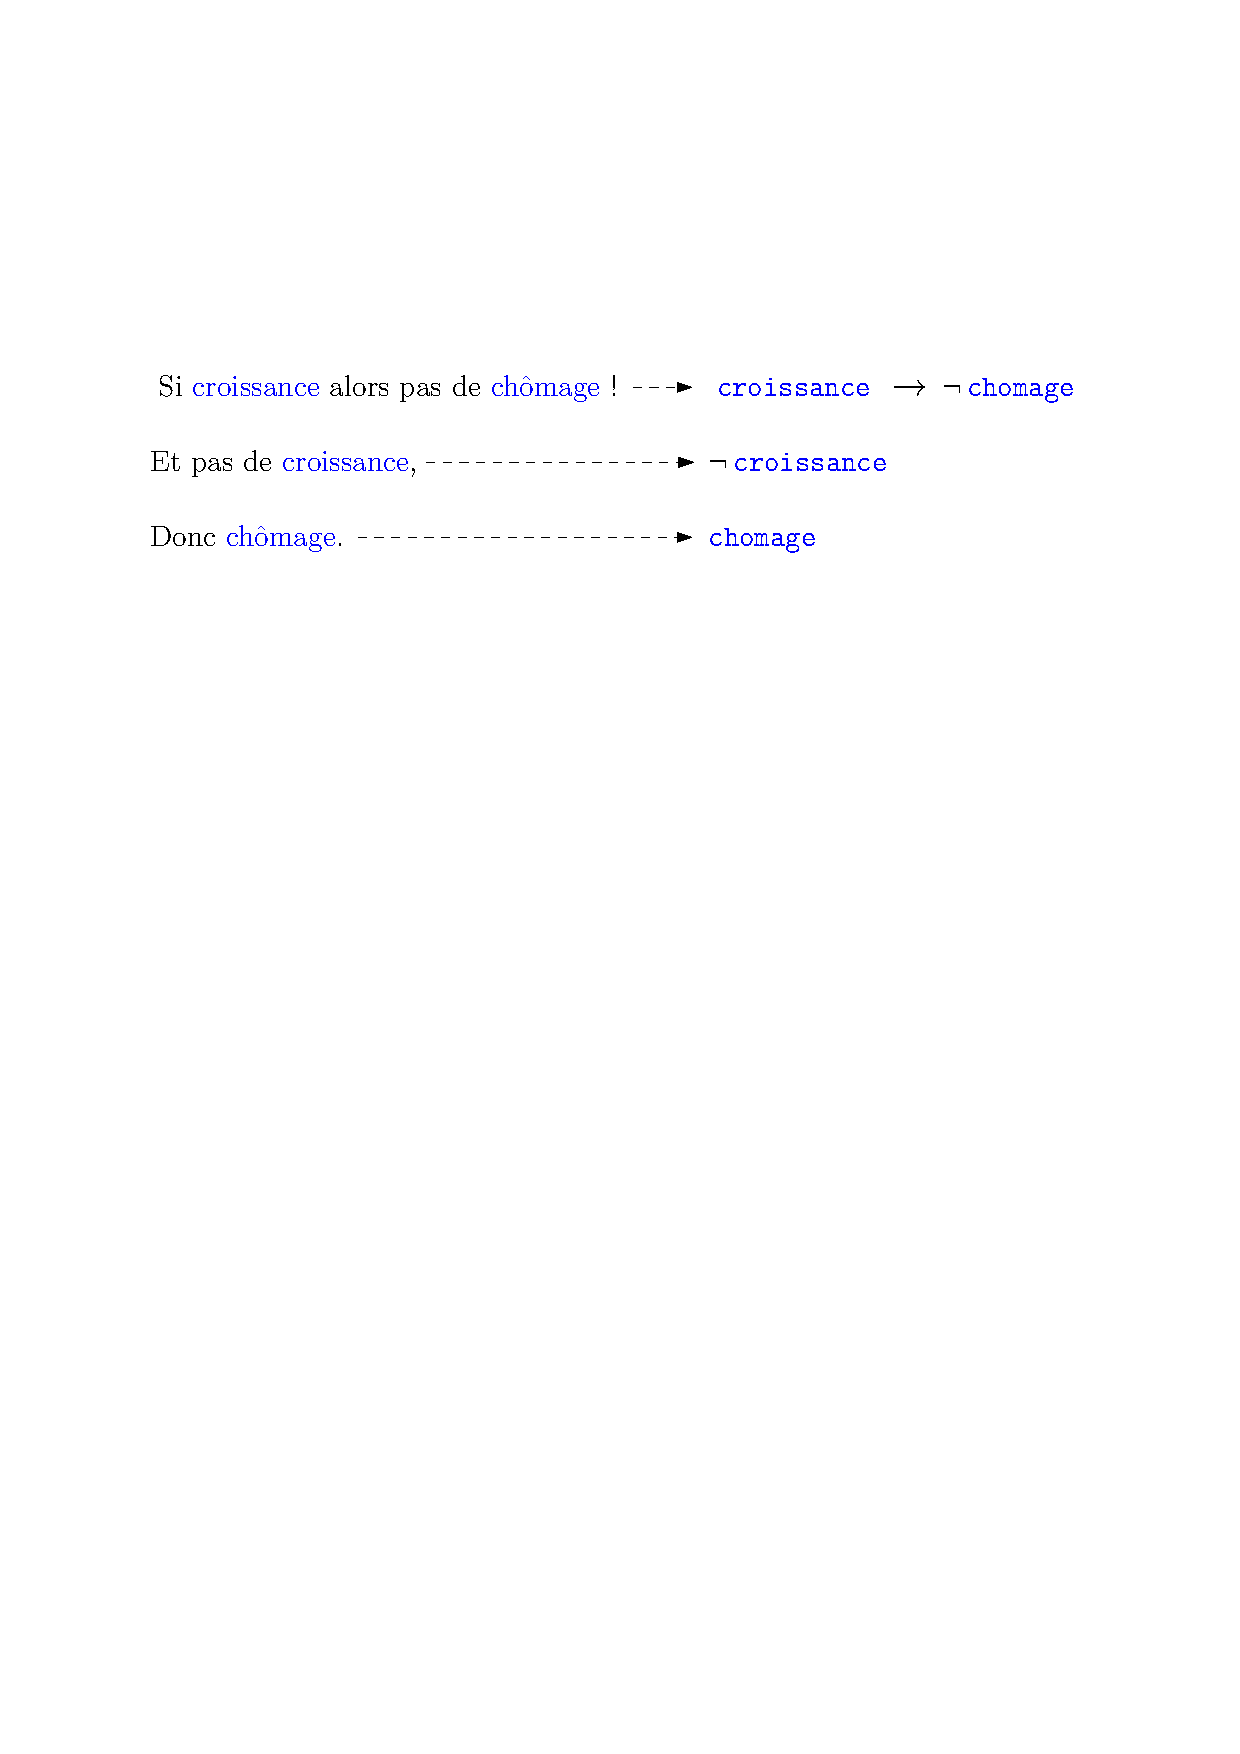
\includegraphics[width=0.95\paperwidth]{figures/intro-logique-1.pdf}}
\end{frame}

\begin{frame}{\subsecname}
\begin{center}\textbf{Étape 2} : poser le problème\end{center}
\begin{block}{Théorème}
\[\{H_1, H_2\} \models C \mbox{ si et seulement si } \{H_1, H_2\} \cup \{\neg C\} \text{insatisfiable}\]
\end{block}
\makebox[\textwidth]{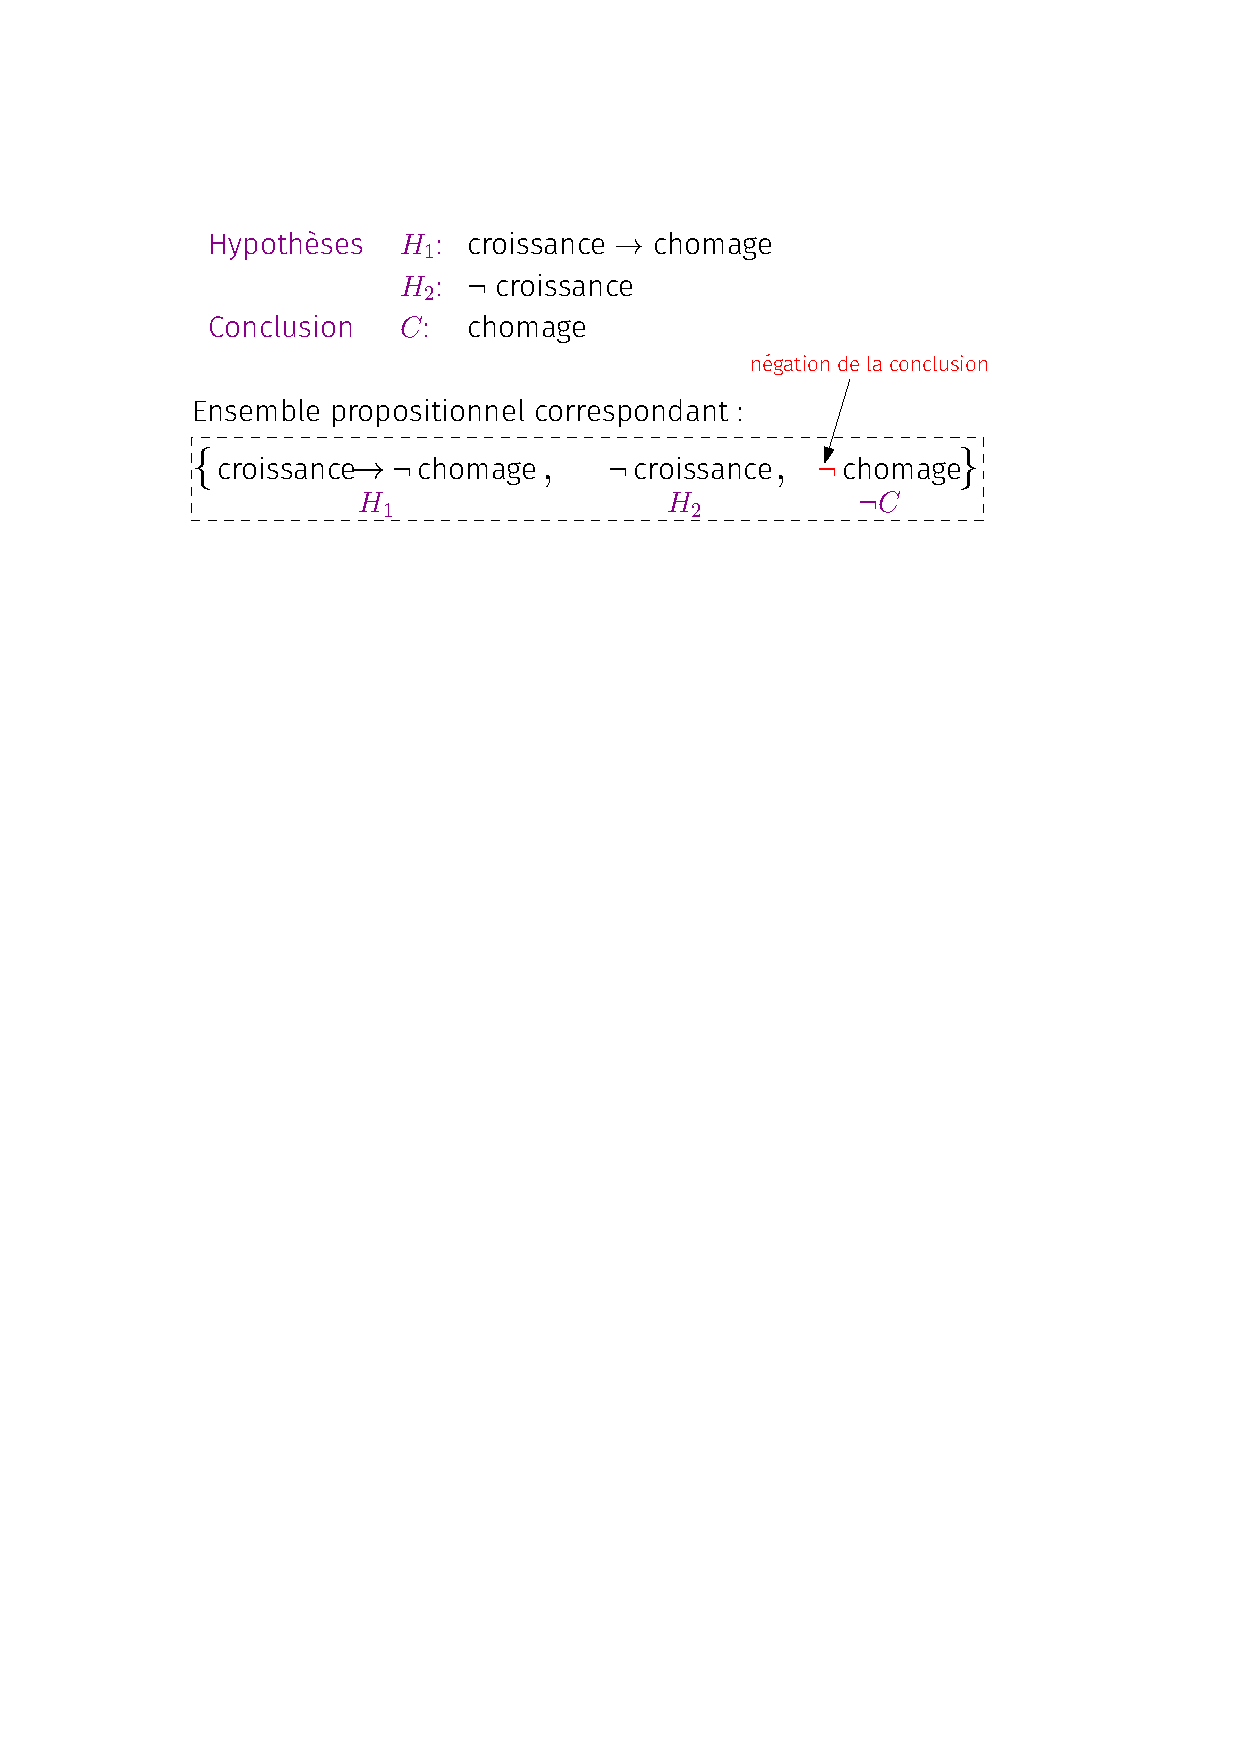
\includegraphics[width=0.95\paperwidth]{figures/intro-logique-2.pdf}}
\end{frame}

% aucun moyen de rendre la formule vraie
\begin{frame}{\subsecname}
\begin{center}\textbf{Étape 3} : résoudre (principe)\end{center}
\begin{block}{Définition d'un problème SAT}
Existe t-il une \emph{valuation} de l'ensemble de formules qui soit \emph{modèle} de celui-ci ?
\end{block}

\textbf{Dans notre cas} : le raisonnement du politicien est \textbf{valide},  ssi TouIST ne trouve \textbf{aucun modèle} (i.e., \emph{insatisfiable}).
\end{frame}

\begin{frame}{\subsecname}
\begin{center}\textbf{Étape 3} : résoudre (programme TouIST)\end{center}
\makebox[\textwidth]{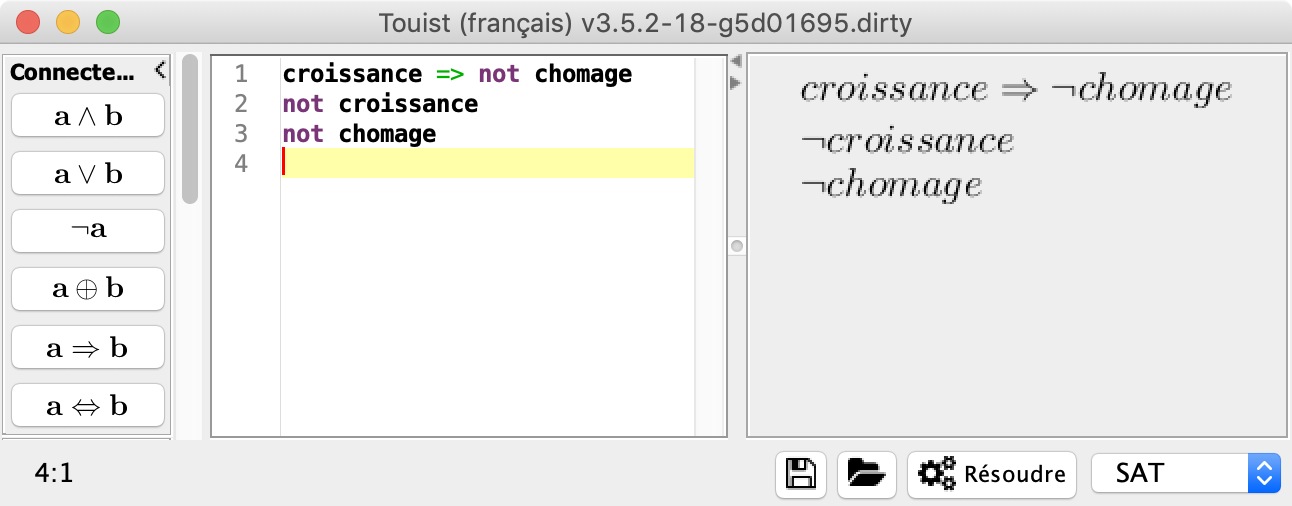
\includegraphics[width=0.9\paperwidth]{figures/touist-policien-1.png}}
\end{frame}

\begin{frame}{\subsecname}
\makebox[\textwidth]{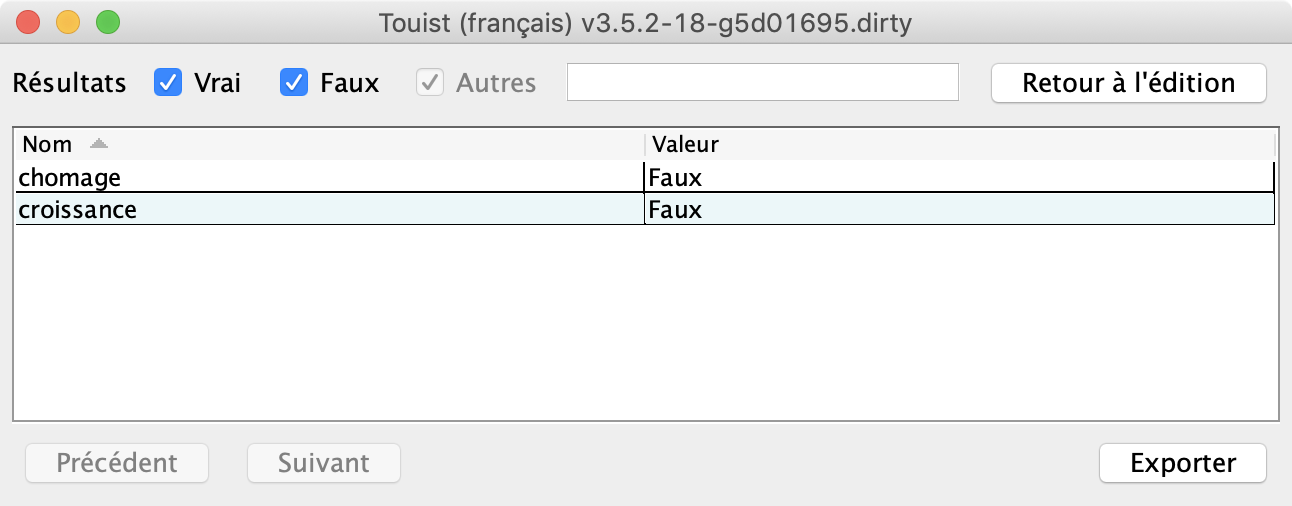
\includegraphics[width=0.9\paperwidth]{figures/touist-policien-2.png}}
\vspace{0cm} \\
\textbf{Conclusion} : un modèle trouvé, donc le raisonnement \textbf{n'est pas valide !}
\end{frame}


\subsection{Aspects d'implémentation}


\begin{frame}{\subsecname}

\includegraphics[scale=0.2]{figures/iaf2015/touist_logo.png}
\huge TouIST \normalsize (Toulouse Integrated Satisfiability Tool)\\[2ex]
\begin{center}
Interface graphique d'écriture de formules logiques dans un \textbf{langage compact} et faisant appel à différents \textbf{solveurs externes}.
\end{center}
\begin{itemize}
    \item sous licence MIT, sources : \url{github.com/touist/touist}
    \item interface graphique (\textbf{Java})
    \item traduction vers solveurs gérée par un compilateur (\textbf{OCaml})
    \item compatible \textbf{SAT, SMT et QBF}
\end{itemize}
\end{frame}

% \begin{frame}[containsverbatim]
% Aperçu du langage d'entrée de TouIST :
% \begin{footnotesize}
% \begin{verbatim}
% $Pays = [Italie, France, Espagne]
% $Adjacent(Italie) = [France]
% $Adjacent(France) = [Italie, Espagne]
% $Couleurs = [bleu, rouge]
% bigand $pays, $couleur in $Pays, $Couleurs:
%   color($pays, $couleur) =>
%     bigand $adj, $coul in $Adjacent($pays), diff($Couleurs, [$couleur]):
%       color($adj, $coul)
%     end
% end
% \end{verbatim}
% \end{footnotesize}
% \end{frame}

% \begin{frame}{\subsecname}
% \makebox[\textwidth]{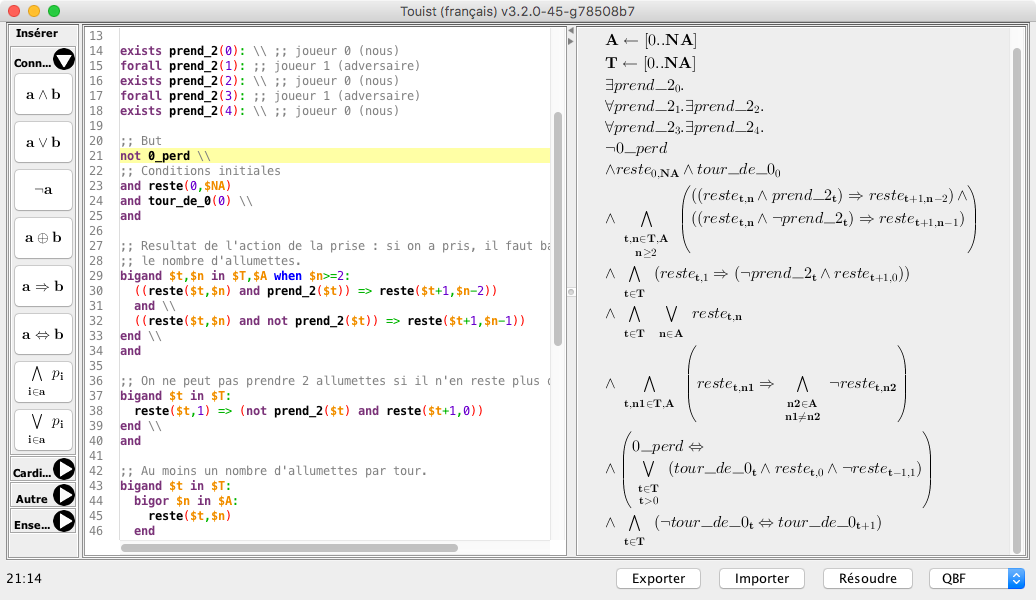
\includegraphics[width=1\paperwidth]{figures/touist-ui.png}}\\
% \end{frame}

\begin{frame}{\subsecname}
\begin{block}{Choix du solveur à la volée}
TouIST permet de choisir le solveur à cibler. Le langage d'entrée s'adapte à chaque solveur.
\end{block}
\begin{center}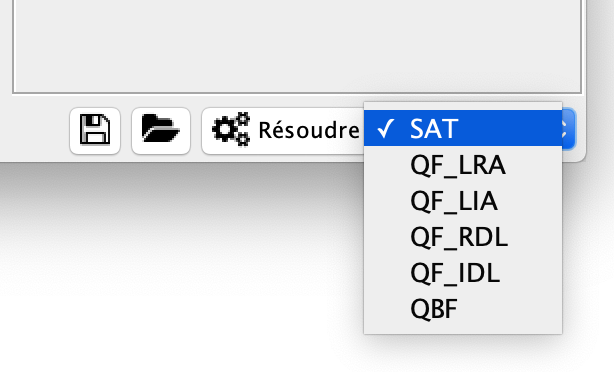
\includegraphics[width=0.6\textwidth]{figures/touist-selecteur.png}\end{center}
\end{frame}

\begin{frame}[containsverbatim]{\subsecname}
Langage d'entrée de TouIST :
\begin{itemize}
    \item \alert{variables} et \alert{ensembles} \\[5pt]
    \begin{small}\begin{verbatim}
  $N = 5
  $Lignes = [1..$N]
  $Pays = [France, Italie, Espagne]
    \end{verbatim}\end{small}
    \item \alert{connecteurs généralisés} \\[5pt]
    \begin{small}\begin{verbatim}
  en(France) and en(Italie) and en(Espagne)

  bigand $p in $Pays:
    en($p)
  end
    \end{verbatim}\end{small}
\end{itemize}
\end{frame}

\begin{frame}[containsverbatim]{\subsecname}
Solveurs compatibles :
\begin{table}
    \centering
    \begin{tabular}{l|l|l}
        \textbf{Solveur} & \textbf{Formule} & \textbf{Équivalent TouIST} \\[5pt]
SAT
&
$a \wedge b \rightarrow c$
&
\begin{minipage}{4cm}\begin{verbatim}
a and b => c
\end{verbatim}\end{minipage}
\\[5pt]

SMT {\scriptsize{}(QF-LIA)}
&
$(x + y - z \ge 4) \vee b$
&
\begin{minipage}{4cm}\begin{verbatim}
(x + y - z >= 4) or a
\end{verbatim}\end{minipage}
\\

SMT {\scriptsize{}(QF-LRA)}
&
$(x + y - z > 4.0) \rightarrow c$
&
\begin{minipage}{5cm}\begin{verbatim}
(x + y - z > 4.0) => c
\end{verbatim}\end{minipage}
\\

SMT {\scriptsize{}(QF-IDL)}
&
$(x - y > 2) \wedge c$
&
\begin{minipage}{5cm}\begin{verbatim}
(x - y > 2) and c
\end{verbatim}\end{minipage}
\\

SMT {\scriptsize{}(QF-RDL)}
&
$(x - y > 1.0) \wedge c$
&
\begin{minipage}{5cm}\begin{verbatim}
(x - y > 1.0) and c
\end{verbatim}\end{minipage}
\\[5pt]

QBF
&
$\forall b.  a \wedge b$
&
\begin{minipage}{5cm}\begin{verbatim}
forall b: a and b
\end{verbatim}\end{minipage}

    \end{tabular}
\end{table}
\vspace{0.5cm}
\begin{scriptsize}
\begin{itemize}
    \item[] QF-LIA = Quantifier-Free Linear Integer Arithmetic
    \item[] QF-LRA = Quantifier-Free Linear Real Arithmetic
    \item[] QF-IDL = Quantifier-Free Integer Difference Logic
    \item[] QF-RDL = Quantifier-Free Real Difference Logic
\end{itemize}

\end{scriptsize}
\end{frame}


\begin{frame}{\subsecname}
\begin{itemize}
    \item[\plus] Extension Visual Studio Code publiée : \textbf{301 utilisateurs !}
\end{itemize}
\makebox[\textwidth]{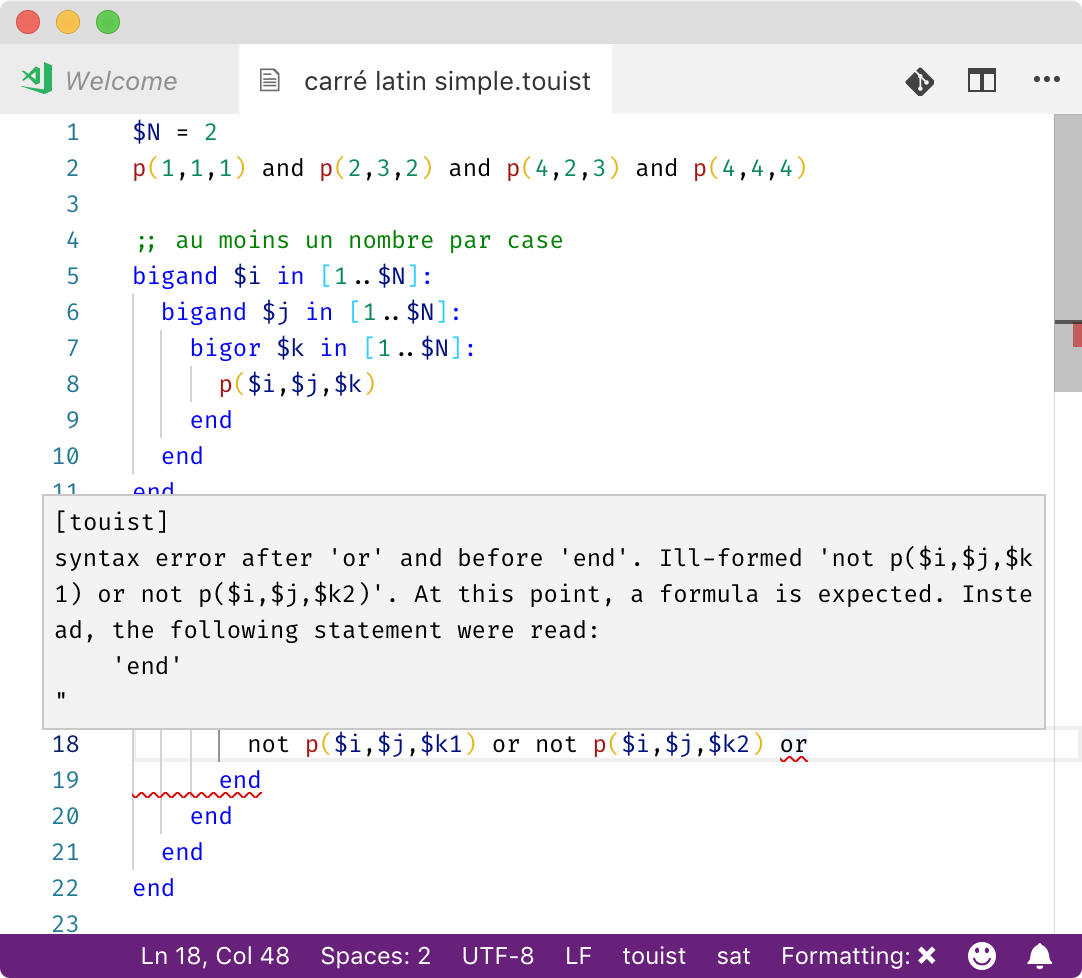
\includegraphics[width=0.5\paperwidth]{figures/vscode-touist-white-with-err}}
\begin{itemize}
    \item[\plus] Et même un plugin Vim ! 
\includegraphics[height=2em]{figures/vim.png}
\end{itemize}
\end{frame}

\begin{frame}{\subsecname}
\begin{itemize}
\item[\plus] Une application web
\item[\plus] plus besoin d'installer Java !
\end{itemize}
\makebox[\textwidth]{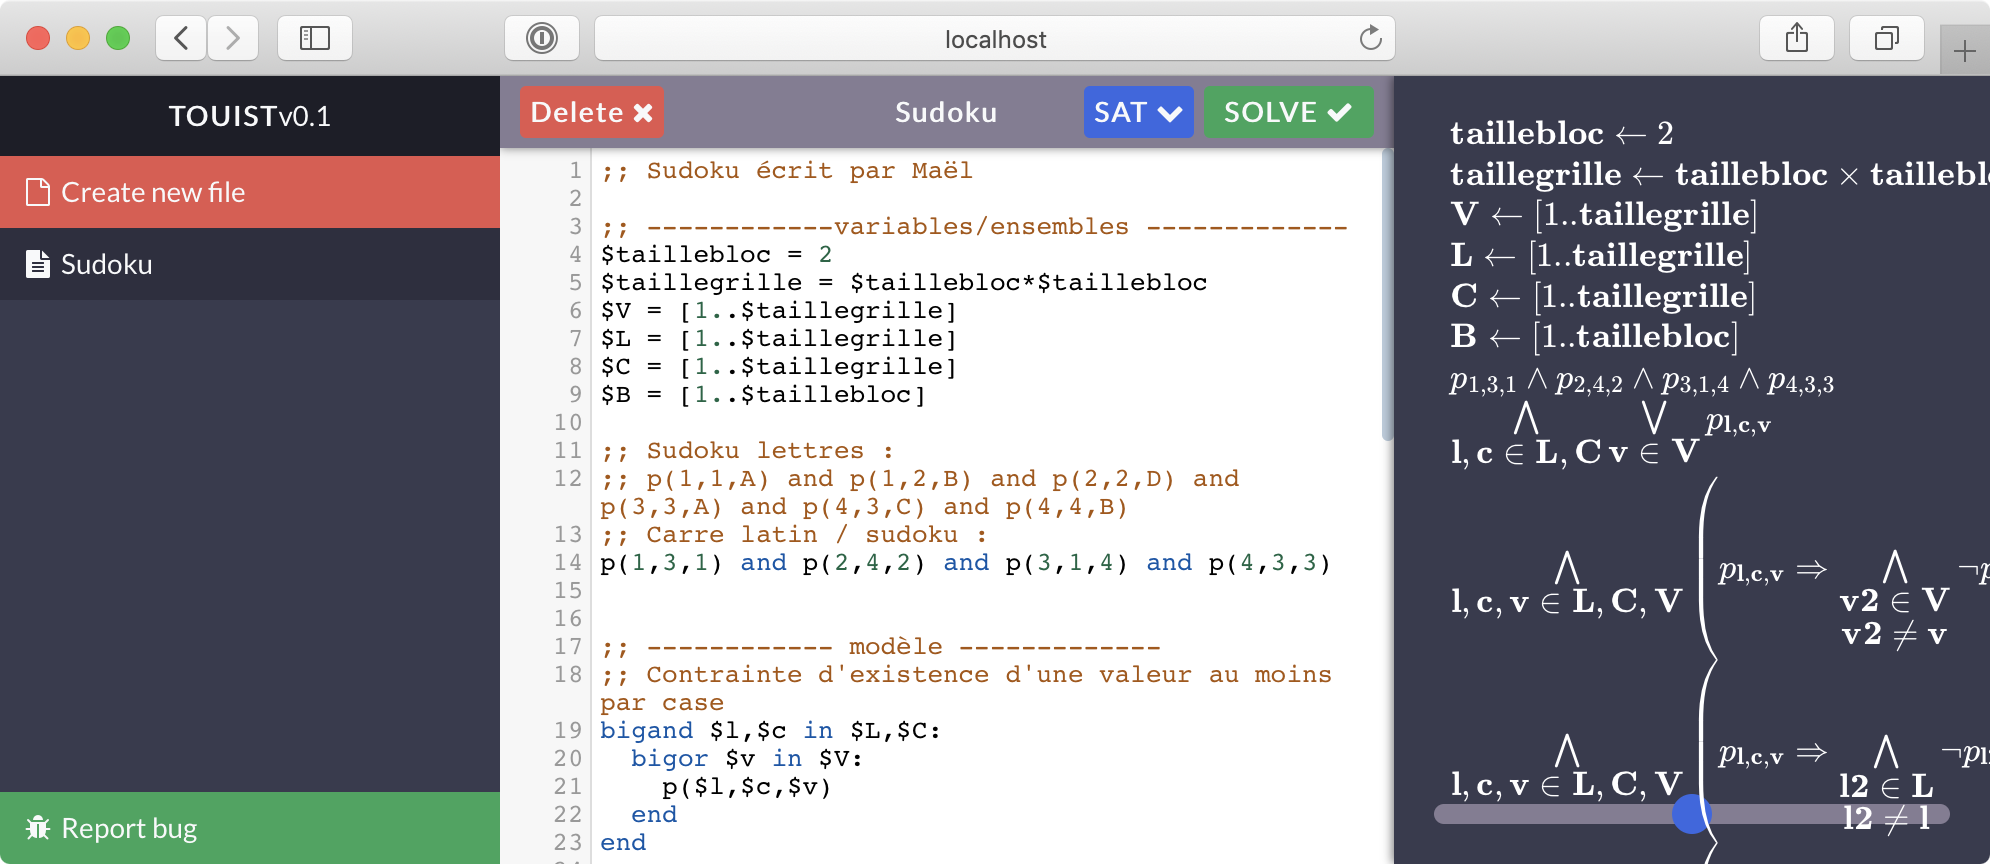
\includegraphics[width=0.9\paperwidth]{figures/touist-web.png}}\\
\end{frame}

% \begin{frame}[containsverbatim]{\subsecname}
% Le compilateur de TouIST en \textbf{OCaml} en mode ligne de commande
% \begin{itemize}
%     \item[\plus] publié sur Opam (OCaml package manager, \cite{Madhavapeddy:2013:URV:2557963.2566628})
%     \item[\plus] compatible avec nombreux solveurs compatibles DIMACS, SMT-LIB et QDIMACS : minisat, picosat, quantor, depqbf, qute...
%     \item[\plus] traduction vers \LaTeX{}
% \end{itemize}
% \begin{block}{Installation et utilisation de la CLI}
% \begin{verbatim}
% opam install touist
% touist - --solve <<< 'pluie => mouille'
% touist --help
% \end{verbatim}
% \end{block}
% \end{frame}


\begin{frame}
\section{II - Utilisation de TouIST avec différents solveurs}
\tableofcontents[currentsection,subsectionstyle=show/show/hide]
\end{frame}


\subsection{Exemple 1 : le Sudoku (SAT)}

\begin{frame}{\subsecname}
\makebox[\textwidth]{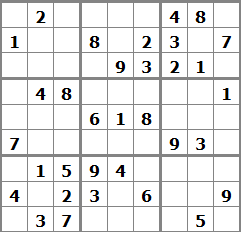
\includegraphics[width=0.5\paperwidth]{figures/iaf2015/sudoku_grille.png}}
\end{frame}


\begin{frame}{\subsecname}
Solution 1 : écrire un \textbf{algorithme \emph{spécifique}}
\begin{itemize}
    \item[\moins] traduction non triviale, développement long
    \item[\moins] maintenance difficile
    \item[\plus] algorithme optimal mais spécifique
\end{itemize}

Solution 2 : utiliser une méthode \textbf{déclarative} (SAT)
\begin{itemize}
    \item[\plus] traduction immédiate des règles
    \item[\plus] meilleure garantie de correction
    \item[\plus] solveurs SAT performants...
    \item[\moins] ...mais moins qu'un algorithme spécifique

\end{itemize}
\end{frame}

\begin{frame}{\subsecname. Étape 1 : modélisation}
\textbf{Étape 1} : modélisation
\makebox[\textwidth]{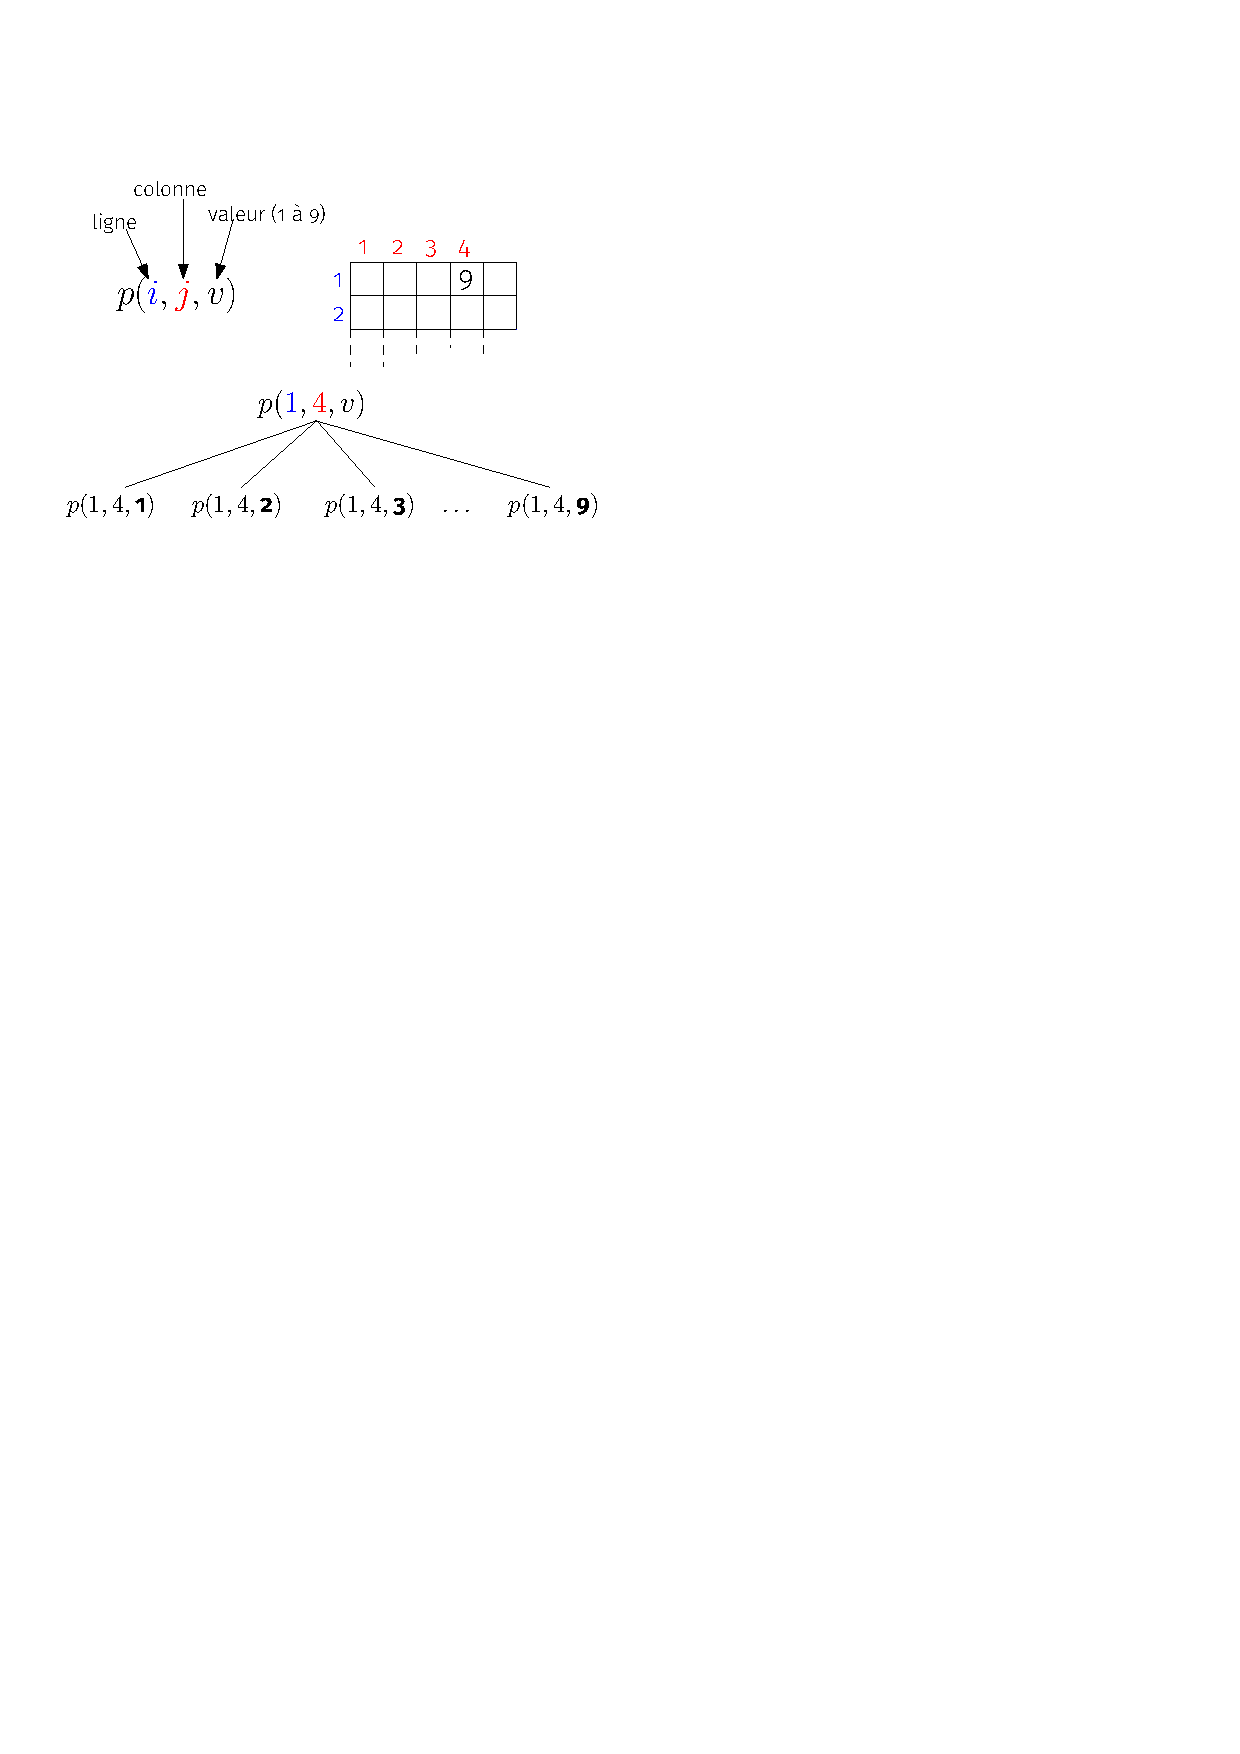
\includegraphics[width=0.7\paperwidth]{figures/sudoku-ligne.pdf}}
\begin{block}{Et maintenant...}
Comment être certain qu'il y a exactement une valeur par case ?
\end{block}
\end{frame}

\begin{frame}[containsverbatim]{\subsecname}
\textbf{Étape 2} : règles (exemple de la case (1,4))
\begin{exampleblock}{Règle 1}
La case (1,4) contient au moins une valeur.
\end{exampleblock}
\[\bigvee_{k\in \text{Valeurs}} \texttt{p(1,4,k)}\]
S'écrit en TouIST :
\begin{small}
\begin{verbatim}
bigor $k in $Valeurs:
  p($i,$j,$k)
end
\end{verbatim}
\end{small}
\end{frame}

\begin{frame}[containsverbatim]{\subsecname. Étape 2 : règles}
\begin{exampleblock}{Règle 2}
Si la case (1,4) a pour valeur 3, alors aucune autre valeur n'est sélectionnée.
\end{exampleblock}
\[\texttt{p(1,4,\hl{3})} \rightarrow \bigwedge_{\substack{k\in [1..9] \\ k\neq 3}} \neg \texttt{p(1,4,\hl{k})} \]
S'écrit en TouIST :
\begin{verbatim}
p(1,4,3) => bigand $k in [1..9] when $k != 3:
              not p(1,4,$k)
            end
\end{verbatim}
\end{frame}



\begin{frame}
\makebox[\textwidth]{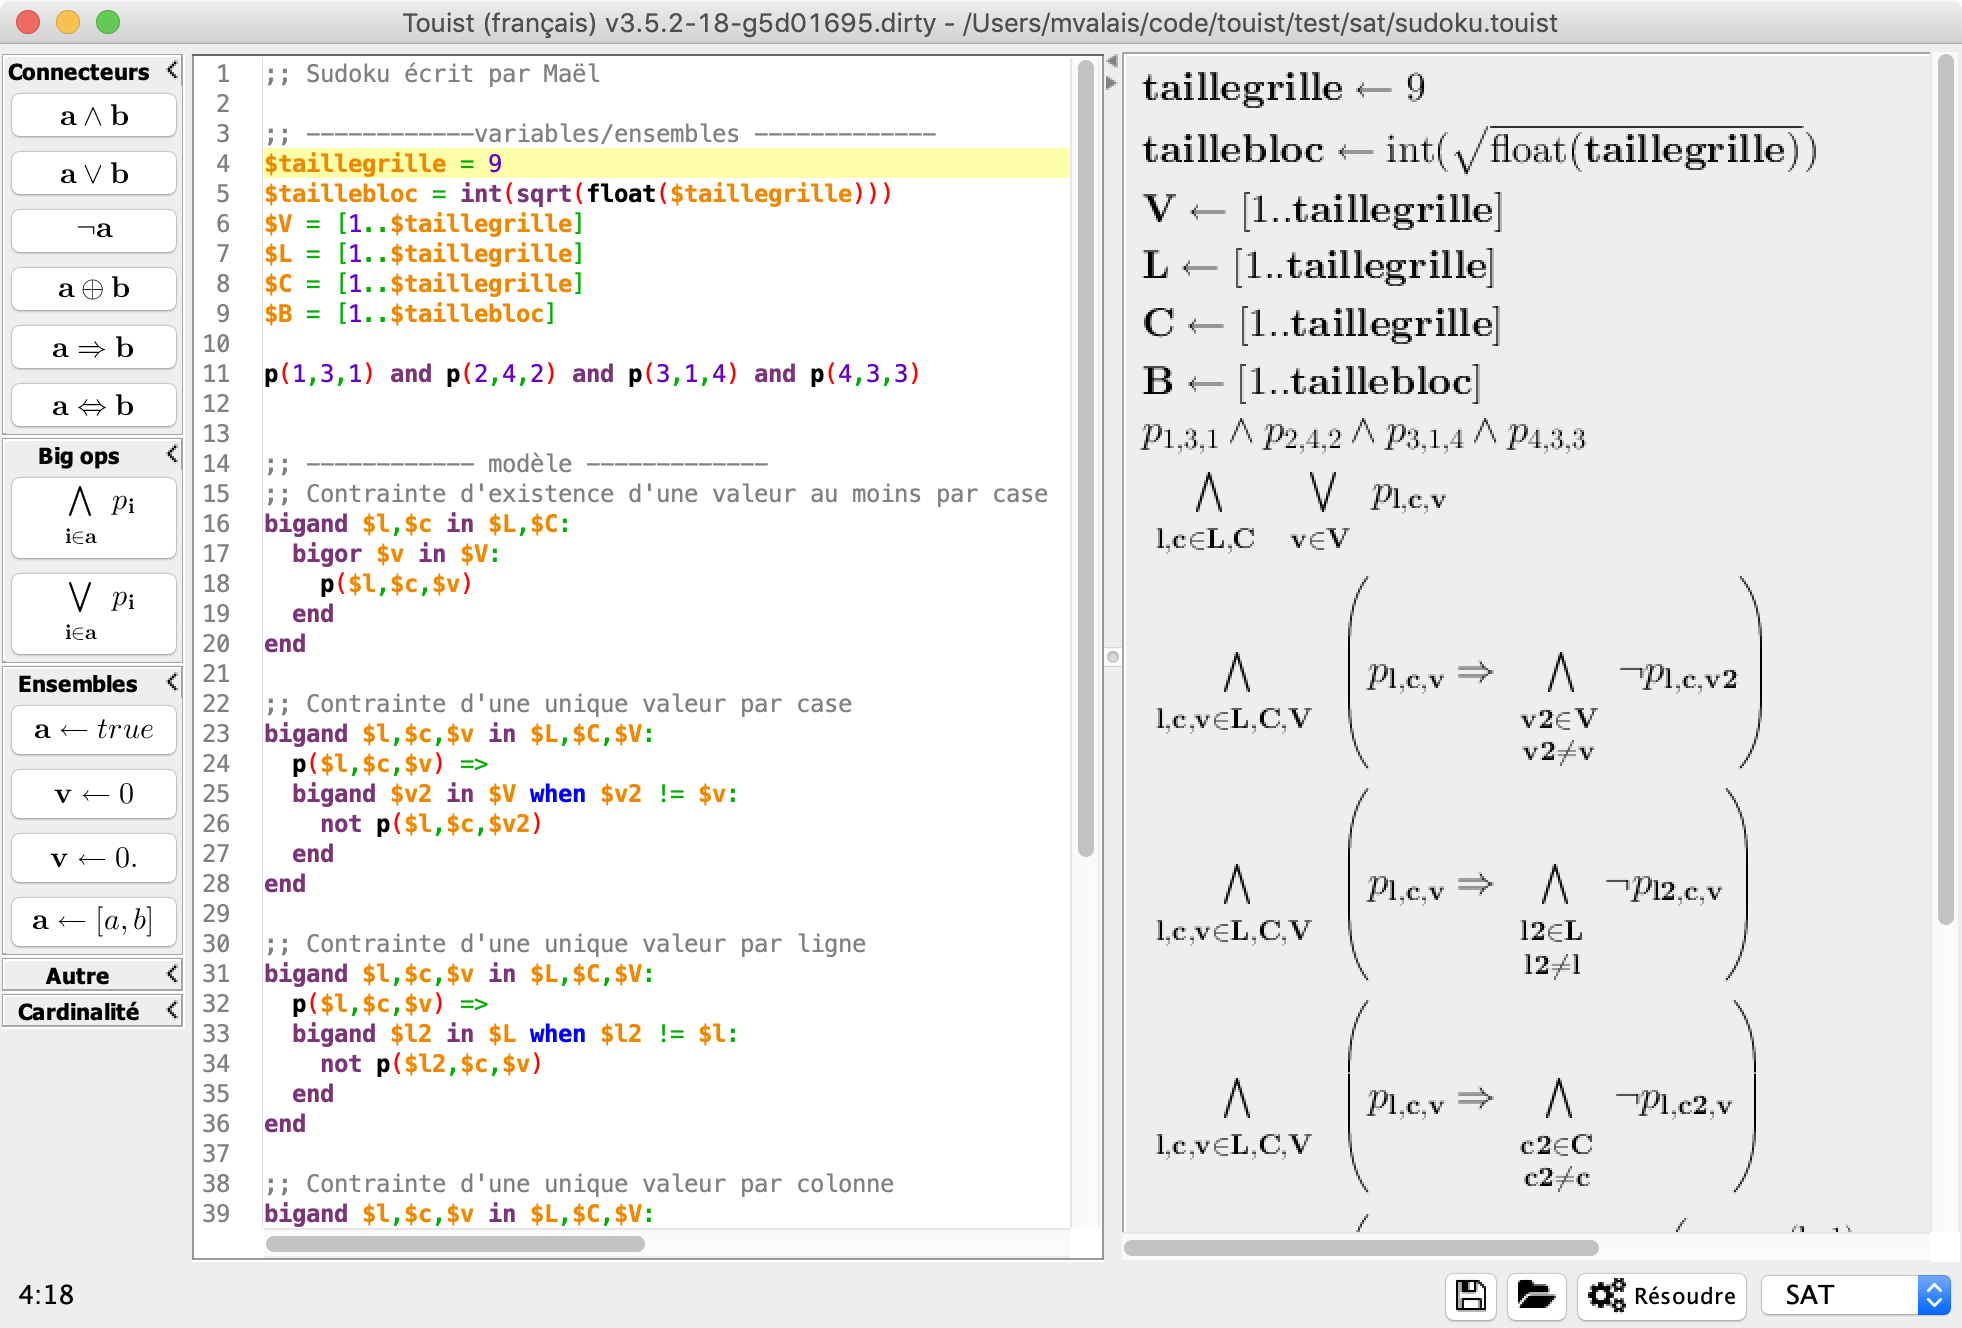
\includegraphics[width=\paperwidth]{figures/touist-sudoku.png}}
\end{frame}

\begin{frame}
\makebox[\textwidth]{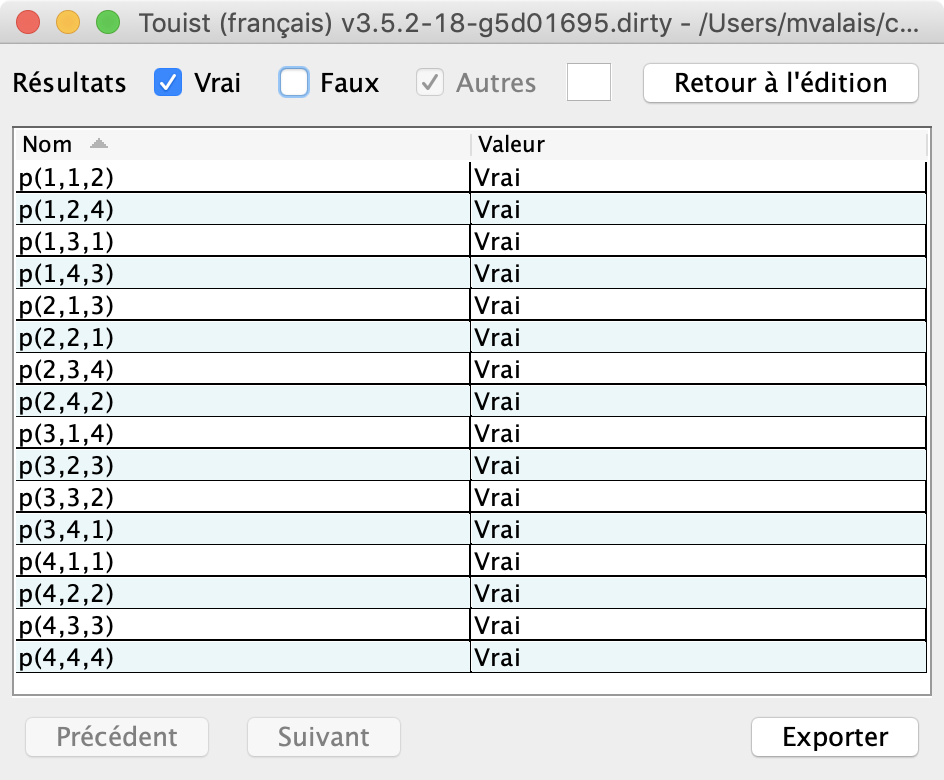
\includegraphics[width=0.8\paperwidth]{figures/touist-sudoku-modele-bis.png}}
\end{frame}

\subsection{Exemple 2 : le Takuzu (SMT)}

\begin{frame}{\subsecname}
Jeu du Takuzu
\makebox[\textwidth]{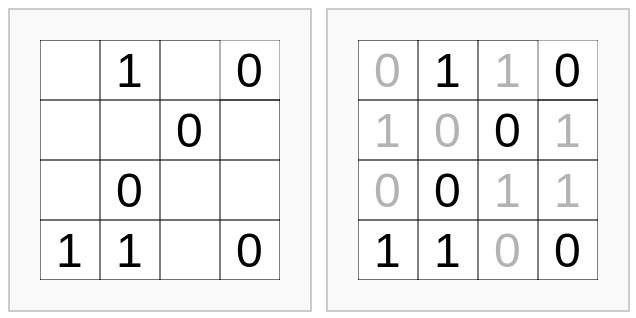
\includegraphics[width=0.8\paperwidth]{figures/iaf2015/Takuzu4x4.png}}
\end{frame}

\begin{frame}[containsverbatim]{\subsecname}
\begin{exampleblock}{Règle 1}
La somme d'une ligne/colonne doit être égale à 2.
\end{exampleblock}

Possible en logique propositionnelle, mais des nécessite \textbf{contraintes de cardinalité} en $O(n^3)$. En SMT :
\begin{verbatim}
bigand $l in $Lignes:
  p($l,1) + p($l,2) + p($l,3) + p($l,4) == 2
end
\end{verbatim}
\end{frame}


\subsection{Exemple 3 : un jeu de Nim (QBF)}

\begin{frame}{\subsecname}
\begin{columns}[T]
\begin{column}{0.3\textwidth}

\includegraphics[width=1\textwidth]{figures/allumettes.png}
\end{column}
\begin{column}{0.7\textwidth}
\begin{exampleblock}{Règles du jeu}
\begin{itemize}
\item 2 joueurs, {\color{ForestGreen}humain} et {\color{red}machine}.
\item Chacun son tour ($t \in T$), un joueur prend 1 à 2 allumettes ($n \in A$).
\item Si un joueur ne peut plus jouer, il a perdu.
\end{itemize}
\end{exampleblock}
\end{column}
\end{columns}
\begin{center}
$\longrightarrow$ Et si on gagnait à \textbf{tous les coups} ?    
\end{center}
\end{frame}

\begin{frame}[containsverbatim]{\subsecname}
\begin{exampleblock}{Règle 1 : \enquote{gagner}}
L'{\color{ForestGreen}humain} gagne ssi il n'existe aucun tour tel que c'est à lui de jouer et il ne reste aucune allumette.
\end{exampleblock}
\[
humain\_gagne \leftrightarrow \neg \bigvee_{\substack{t \in T\\t > 0}}
tour\_de\_humain(t) \wedge reste(t,\alert{0})
\]
\begin{verbatim}
humain_gagne <=>
not bigor $t in $T when $t>0:
 tour_de_humain($t) and reste($t,0)
end
\end{verbatim}
\end{frame}

\begin{frame}[containsverbatim]{\subsecname}
\begin{exampleblock}{Règle 2 : \enquote{jouer}}
Selon son choix, le joueur laisse \alert{une} ou \alert{deux} allumettes en moins.
\end{exampleblock}
\[
\bigwedge_{\substack{t \in T\\ n \in A\\ n \geq 2}} 
\begin{pmatrix}
    (reste(t,n) \wedge prend(t, \alert{2}) \rightarrow reste(t+1,n-\alert{2}))\\
    \wedge (reste(t,n) \wedge prend(t, \alert{1}) \rightarrow  reste(t+1, n-\alert{1}))
\end{pmatrix}
\]
\begin{footnotesize}
\begin{verbatim}
bigand $t,$n in $T,$M when $n>=2:
  ((reste($t,$n) and prend($t,2)) => reste($t+1,$n-2))
 and
  ((reste($t,$n) and prend($t,1)) => reste($t+1,$n-1))
end
\end{verbatim}
\end{footnotesize}
\end{frame}

% \begin{frame}[containsverbatim]{\subsecname}
% \begin{exampleblock}{Règle 3 : "dernier coup"}
% S'il ne reste plus qu'\alert{une} allumette, le joueur n'a pas le choix, il doit la prendre et ne laisse aucune allumette.
% \end{exampleblock}
% \[
% \bigwedge_{\substack{t \in T}} reste(t,\alert{1}) \rightarrow \neg prend\_2(t) \wedge  reste(t+1,\alert{0})
% \]
% \begin{verbatim}
% bigand $t in T:
%   reste($t,1) => not prend_2($t) and reste($t+1,0)
% end
% \end{verbatim}
% \end{frame}

\begin{frame}{\subsecname}
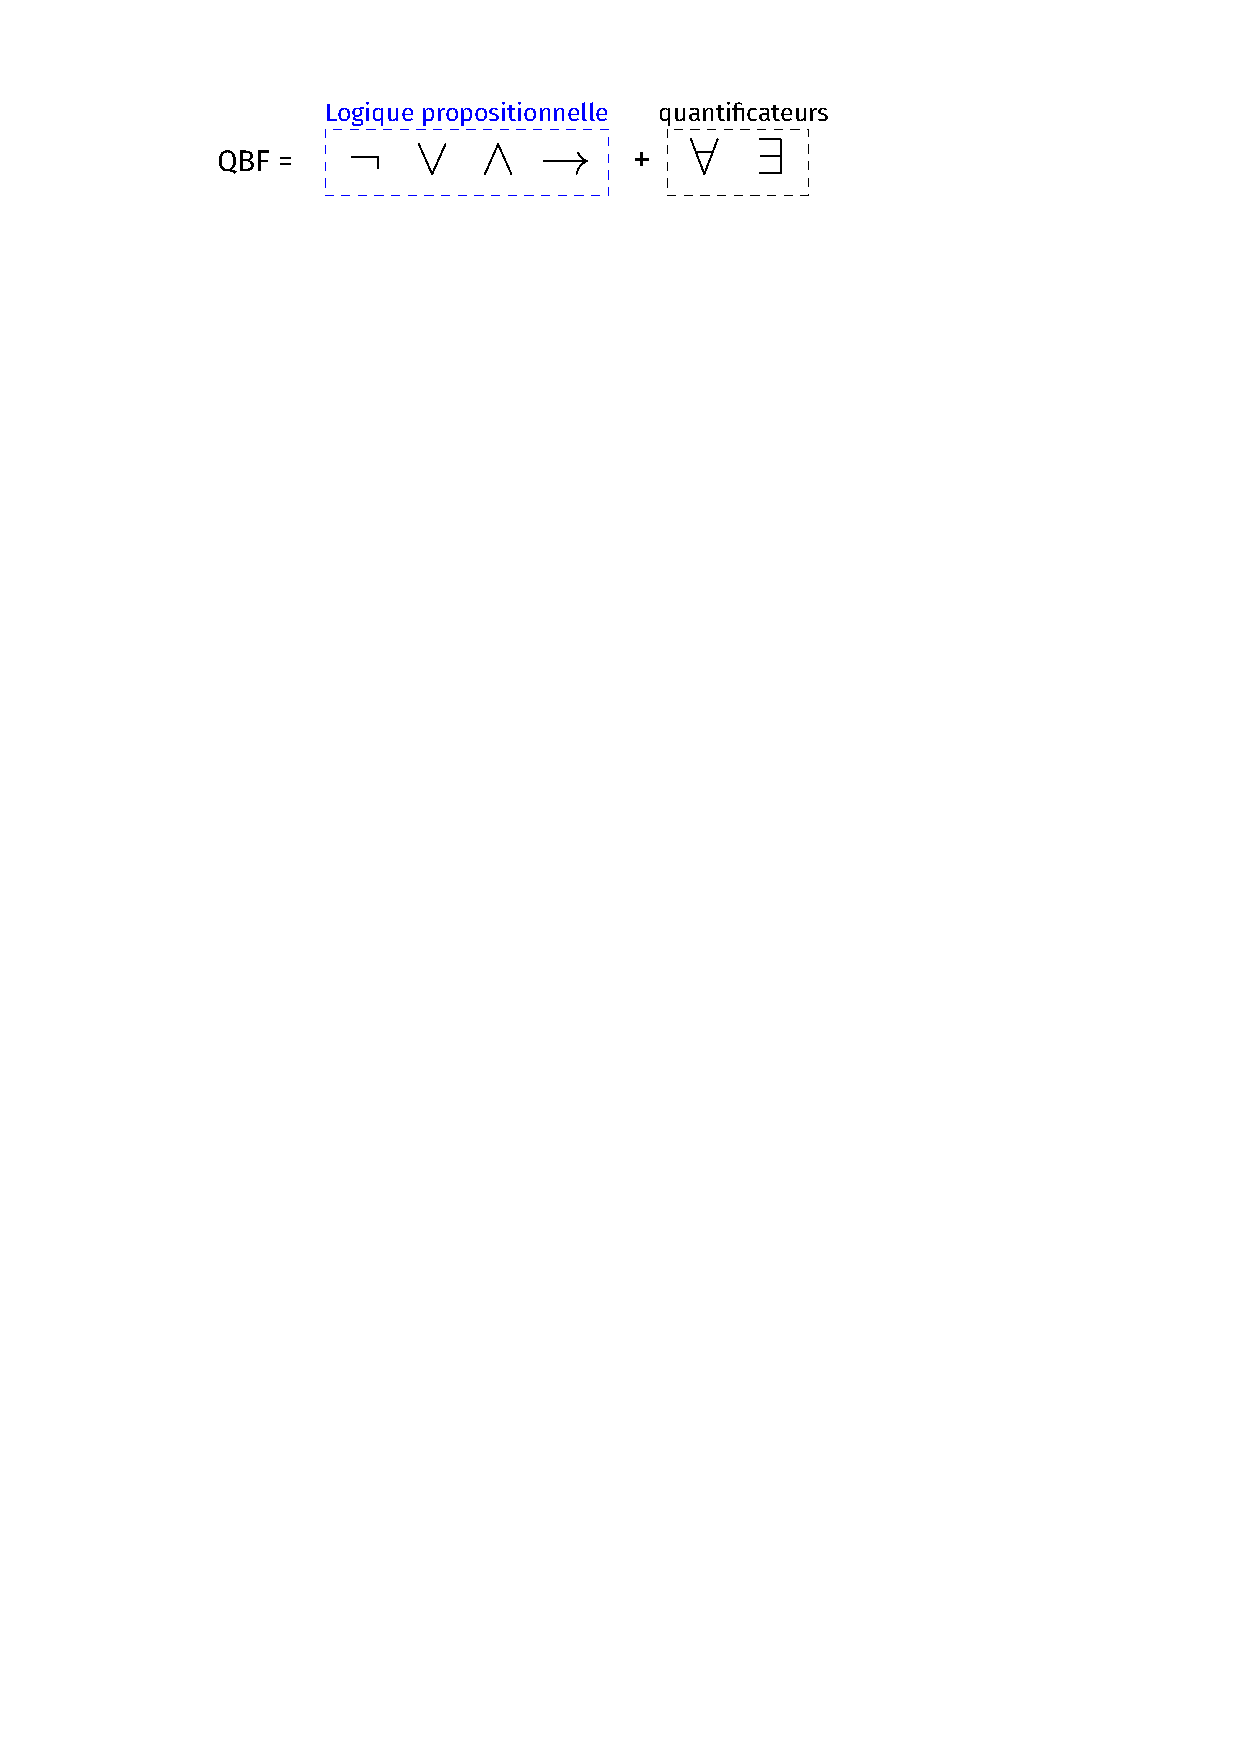
\includegraphics[width=1\textwidth]{figures/nim-arbre-0.pdf} \\ \vspace{0cm}
%Toutes les feuilles sont satisfiables ssi solution du problème TQBF est {vrai}
\end{frame}

\begin{frame}{\subsecname}
Arbre de jeu décrivant une partie
\makebox[\textwidth]{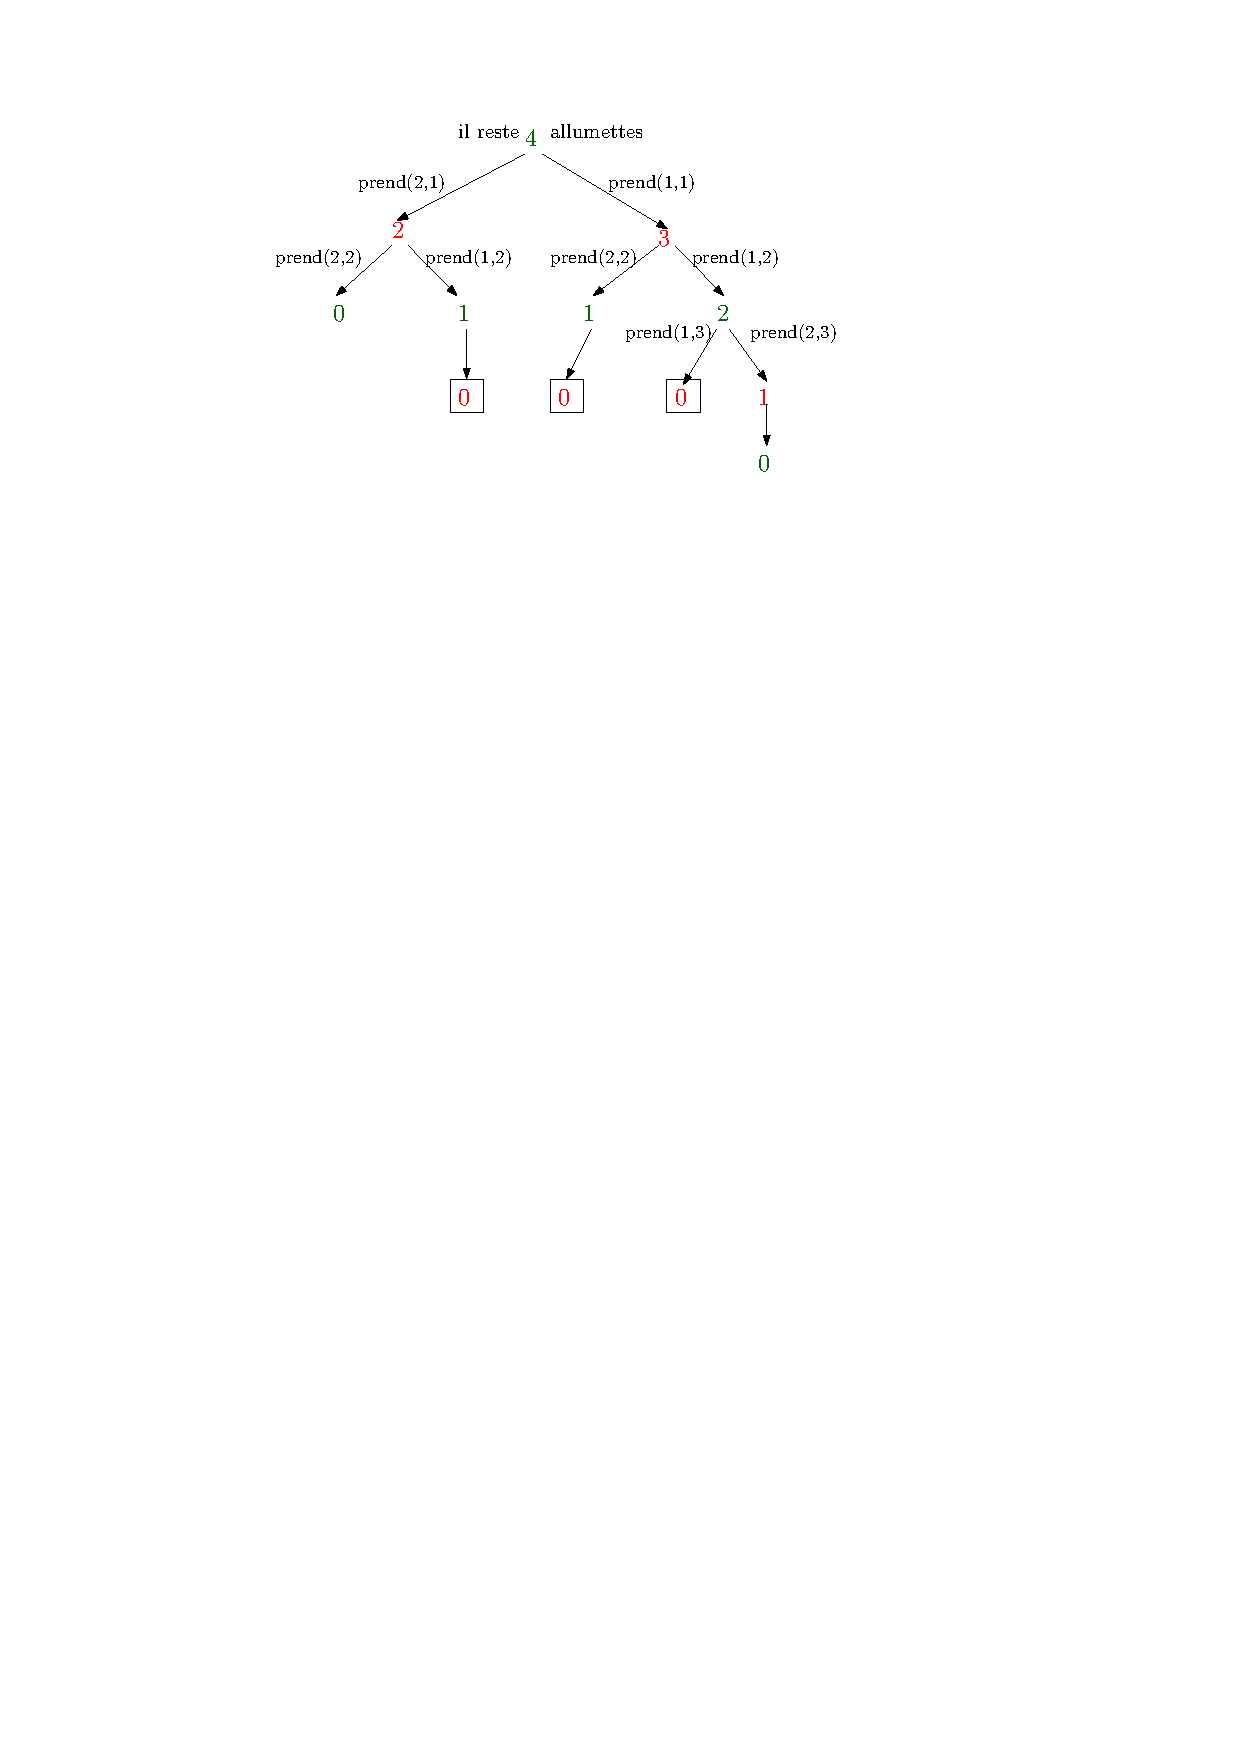
\includegraphics[width=\textwidth]{figures/nim-arbre-1.pdf}}
\end{frame}

\begin{frame}{\subsecname}
Arbre ET/OU
\makebox[\textwidth]{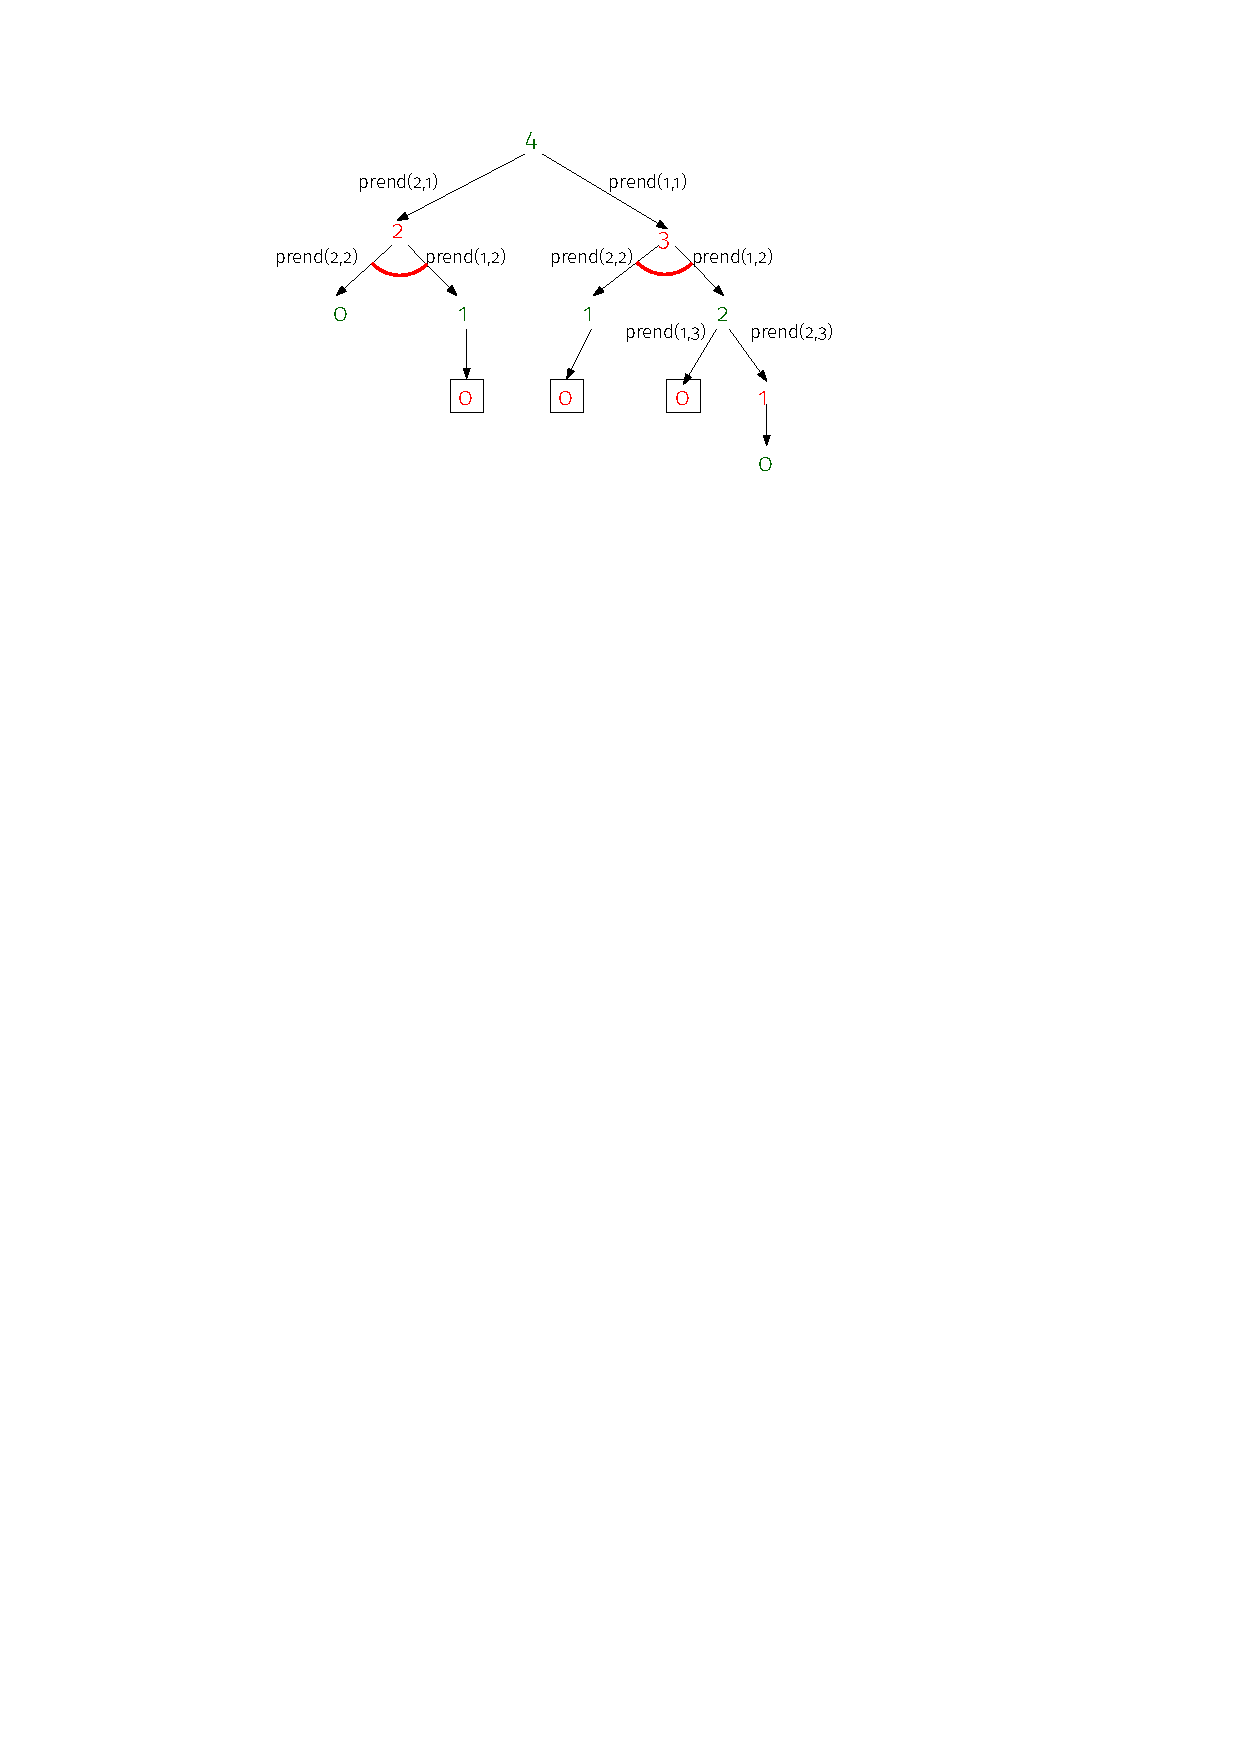
\includegraphics[width=\textwidth]{figures/nim-arbre-2.pdf}}
\end{frame}


\begin{frame}{\subsecname}
Trouver la stratégie gagnante pour le {\color{ForestGreen}joueur humain} (s'il y en a une)
\begin{itemize}
    \item SAT = taille formule exponentielle
    \item QBF = taille formule linéaire
\end{itemize}
\end{frame}

\begin{frame}{\subsecname}
\makebox[\textwidth]{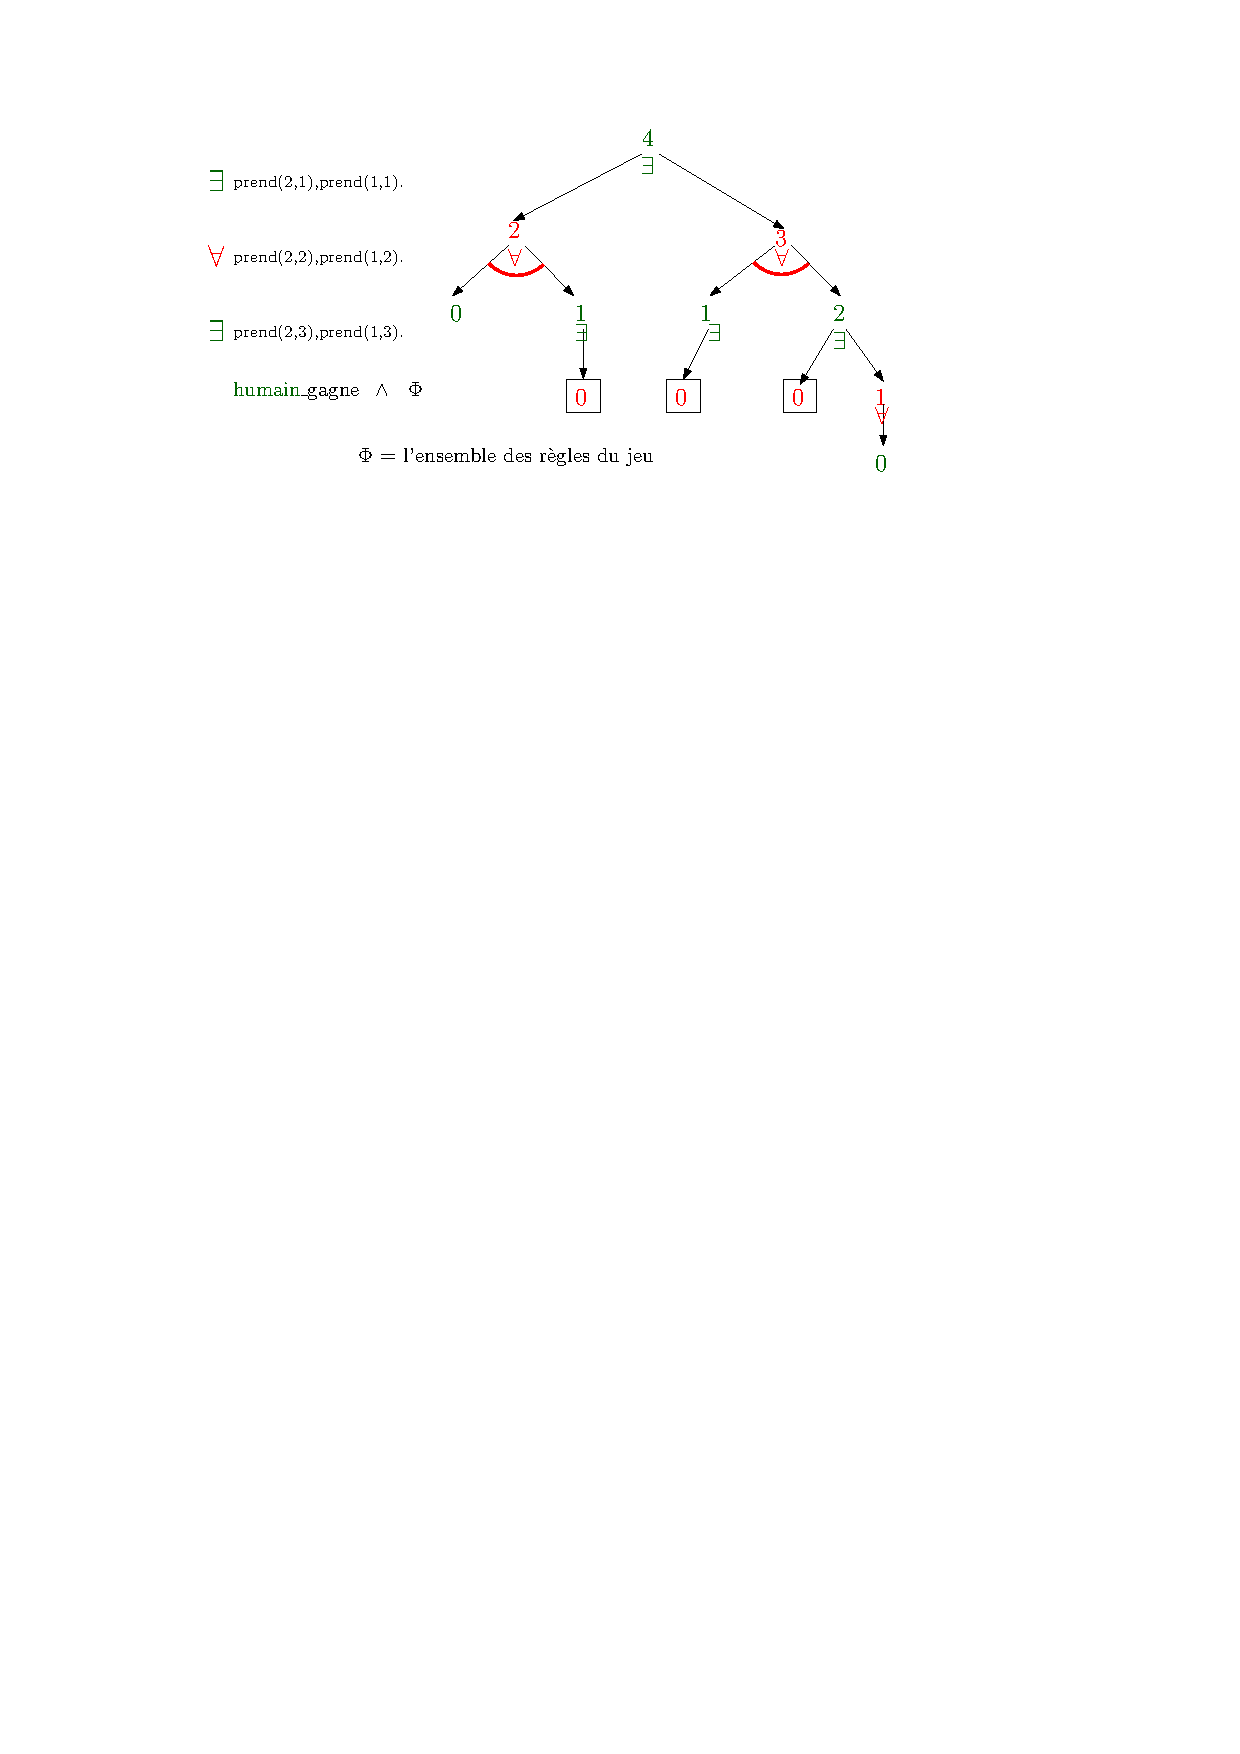
\includegraphics[width=\textwidth]{figures/nim-arbre-3.pdf}}
\end{frame}

\begin{frame}{\subsecname}
\makebox[\textwidth]{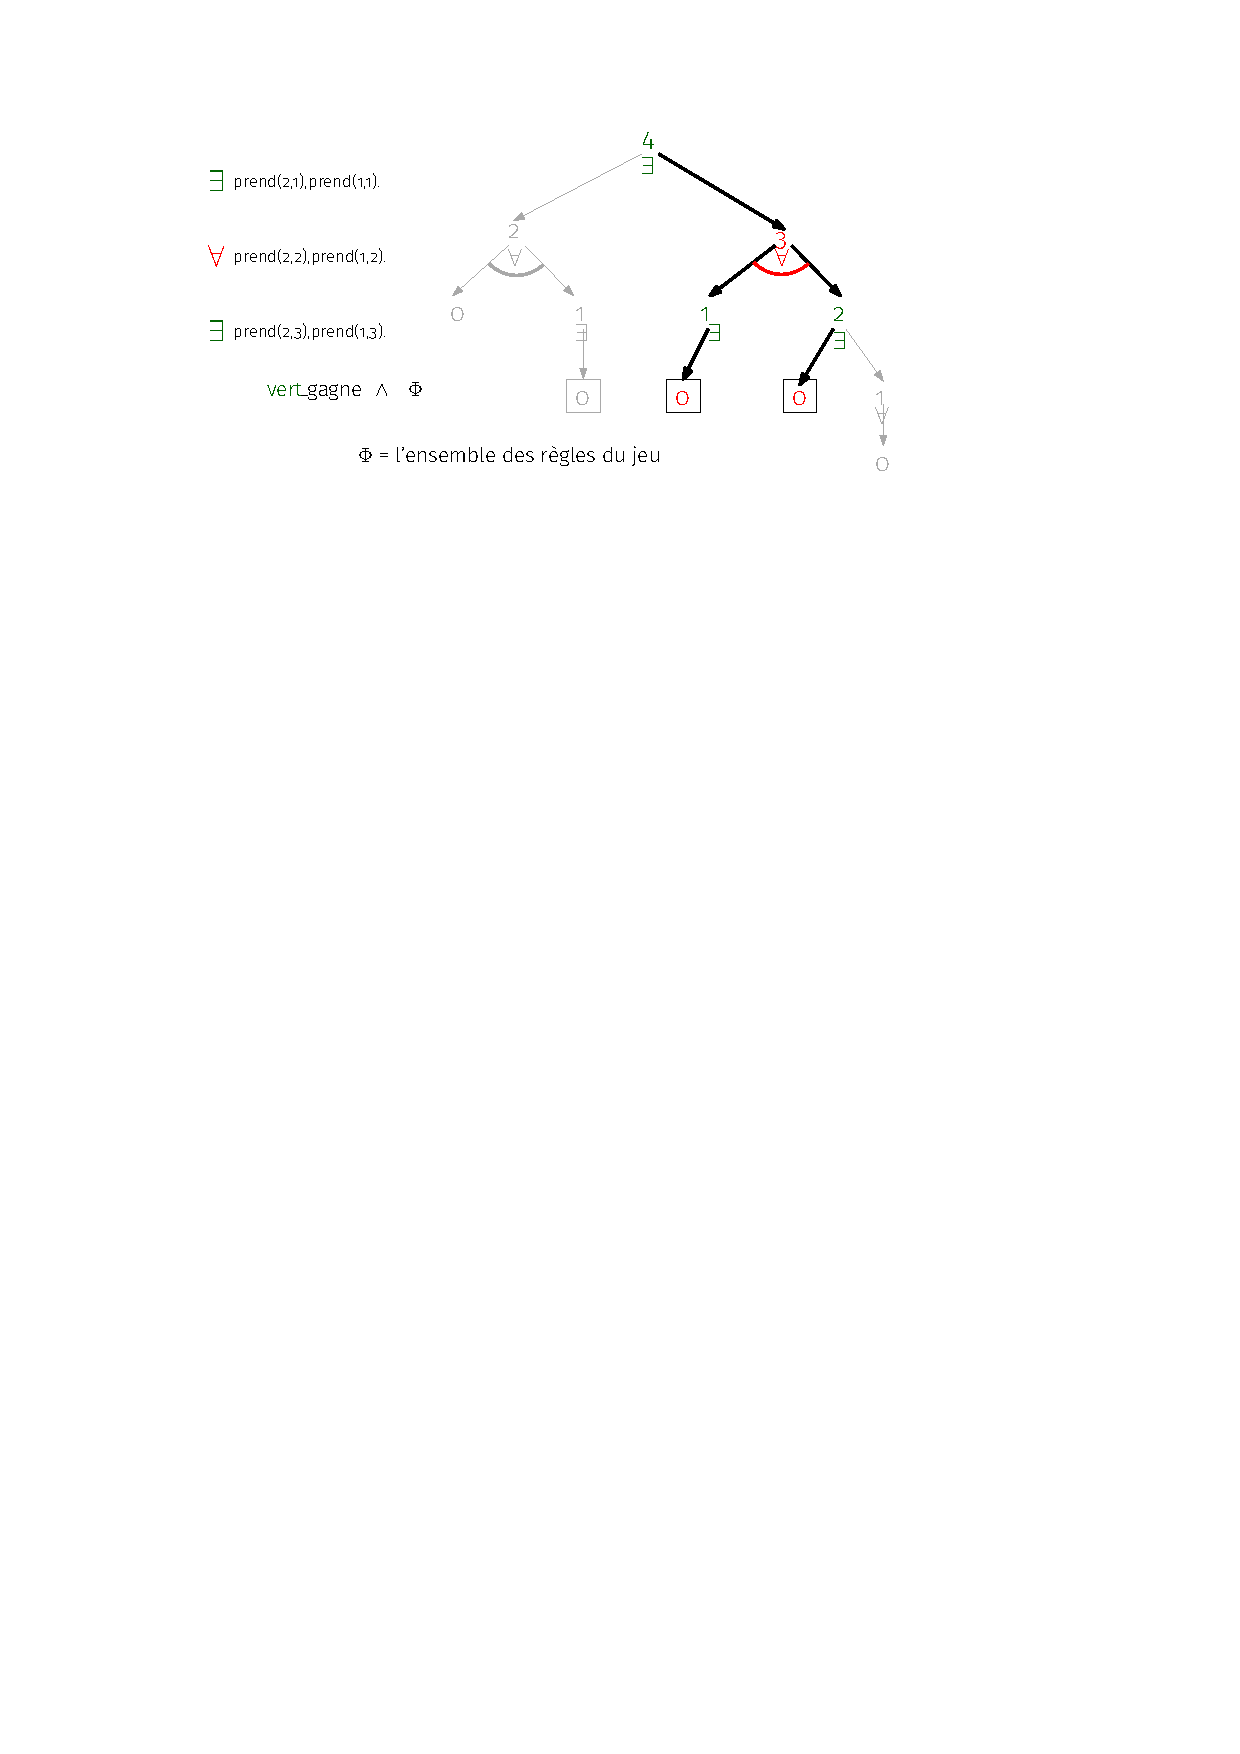
\includegraphics[width=\textwidth]{figures/nim-arbre-4.pdf}}
\end{frame}

\begin{frame}
\section{III - Application à la planification}
\tableofcontents[currentsection,subsectionstyle=show/show/hide]
\end{frame}

\subsection{Planification classique ?}
\begin{frame}{\subsecname}
\begin{columns}[T,onlytextwidth]
\begin{column}{0.45\textwidth}\centering
État initial\\
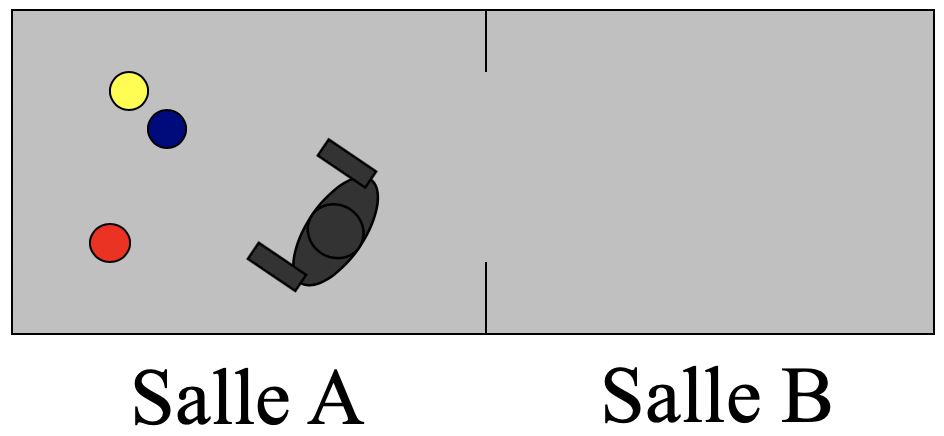
\includegraphics[width=\textwidth]{figures/gripper-start.png}
\end{column}
\begin{column}{0.45\textwidth} \centering
But\\
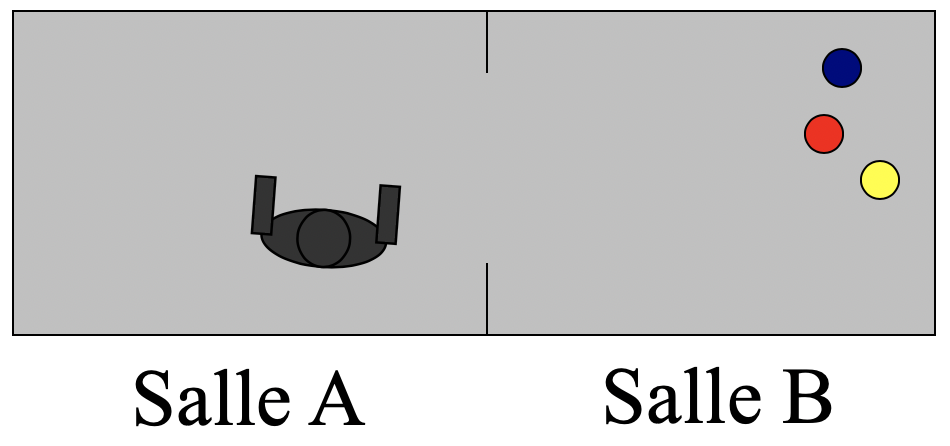
\includegraphics[width=\textwidth]{figures/gripper-end.png}
\end{column}
\end{columns}
\begin{itemize}
    \item Partir de l'\textbf{état initial}
    \item Arriver à un état qui satisfait le \textbf{but}
    \item À partir d'\textbf{actions} {\scriptsize{}(plusieurs actions possibles par étape)} \\[10pt]
\begin{small}\begin{tabular}{l|l}
    PICK(balle1, salleA, gauche) & ramasser balle dans main gauche \\
    PICK(balle1, salleA, droit) & ramasser balle dans main gauche \\[5pt]
    DROP(balle1, salleA, gauche) & lâcher main gauche \\
    DROP(balle1, salleA, droit) & lâcher main droite \\[5pt]
    MOVE(salleA, salleB) & aller dans l'autre pièce
\end{tabular}\end{small}
\end{itemize}
\end{frame}

\begin{frame}
Pourquoi exploiter QBF pour la planification ?
\begin{itemize}
\item Un \textbf{article prometteur}, \cite{DBLP:conf/ecai/CashmoreFG12}
\item les compétitions des solveurs QBF attirent \textbf{de plus en plus l'attention}
\item \textsc{Satplan}~ gagne les compétitions IPC'04 et IPC'06 \nocite{KAU04,KSH06} grâce aux amélioration des solveurs SAT \textbf{provoquées par les compétitions}
\end{itemize}

\begin{center}
$\longrightarrow$ les solveurs QBF deviennent de plus en plus performants
\end{center}
\end{frame}

\begin{frame}{\subsecname}
\begin{block}{Définition}
Plan = séquence d'\textbf{étapes} constituées d'\textbf{actions}.
\end{block}
\makebox[\textwidth]{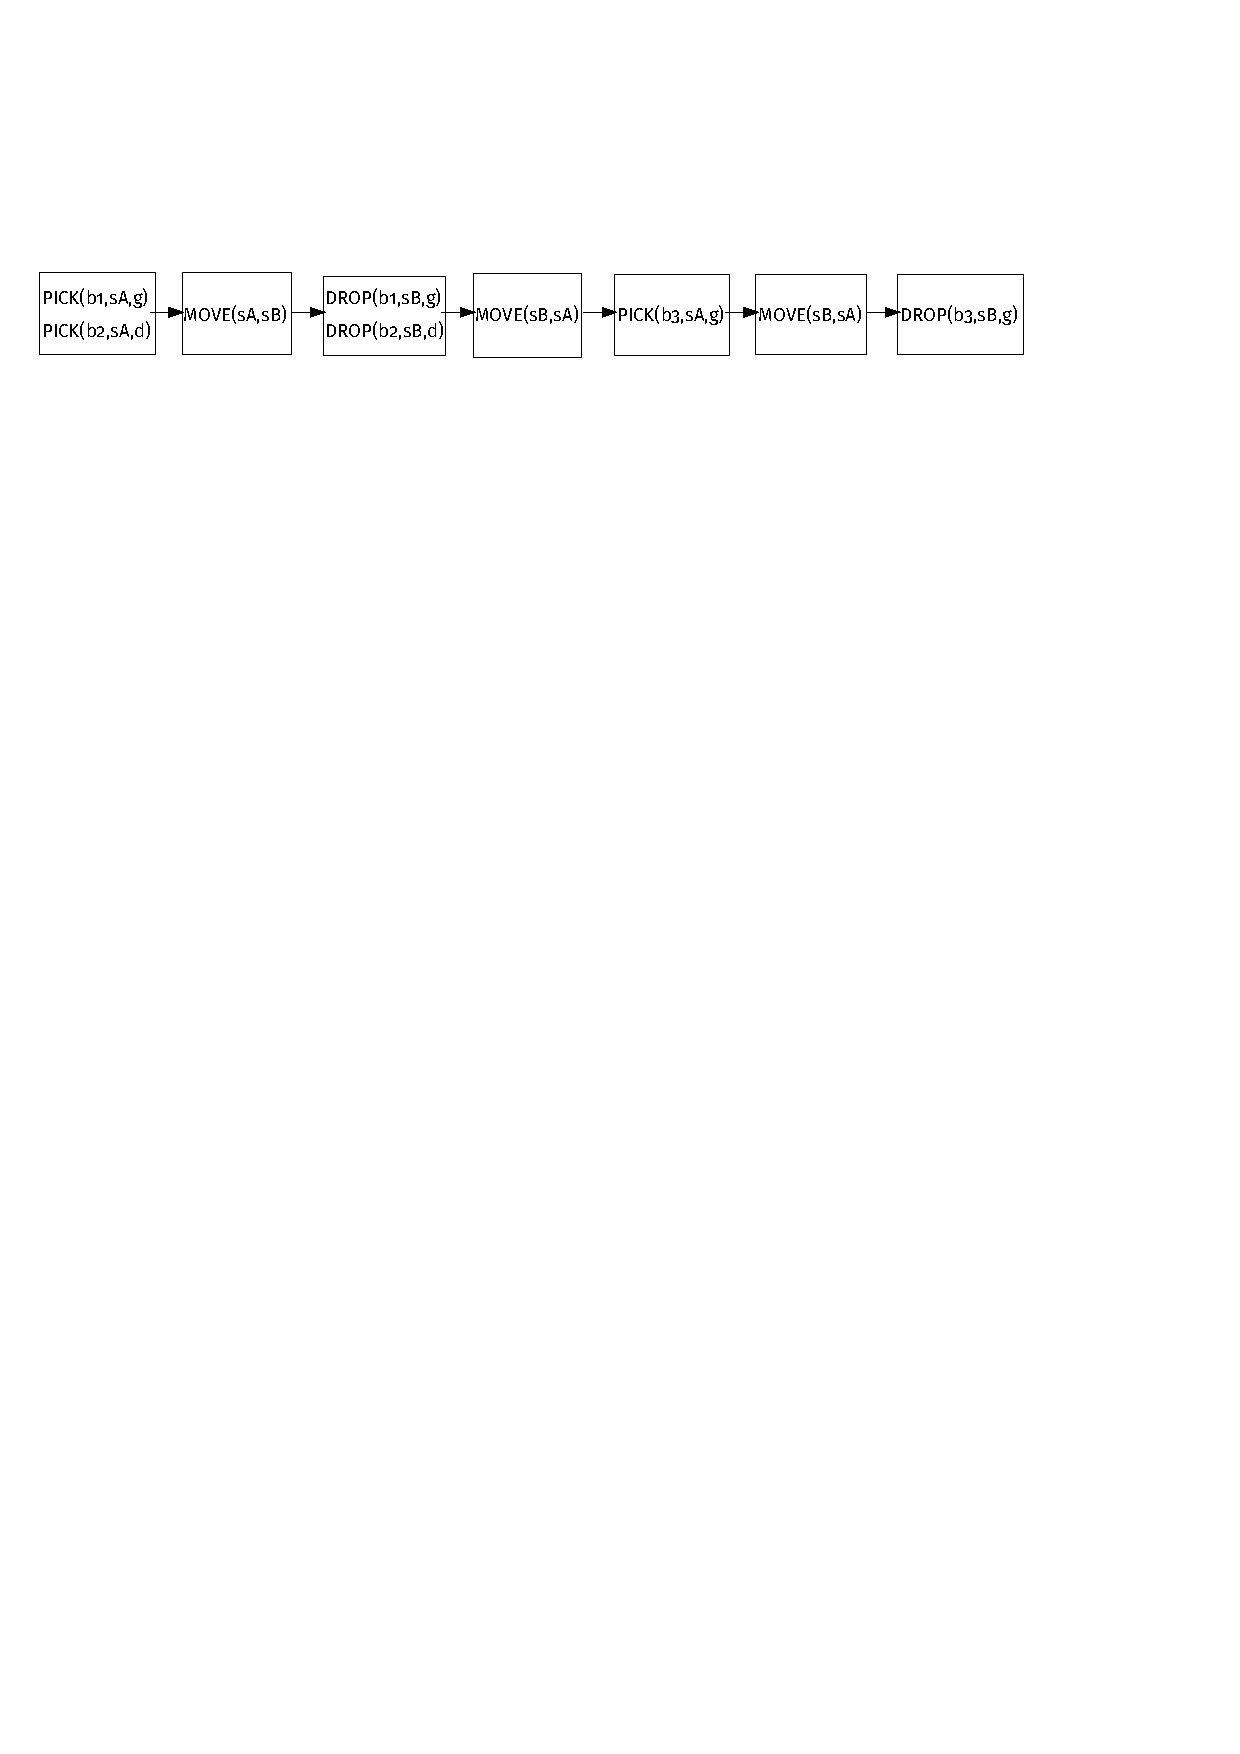
\includegraphics[width=0.98\paperwidth]{figures/plan-gripper.pdf}}
\end{frame}


\begin{frame}{\subsecname}
\textbf{Étape 1} : traduire le problème de planification en problème SAT \\ \vspace{1cm}
\makebox[\textwidth]{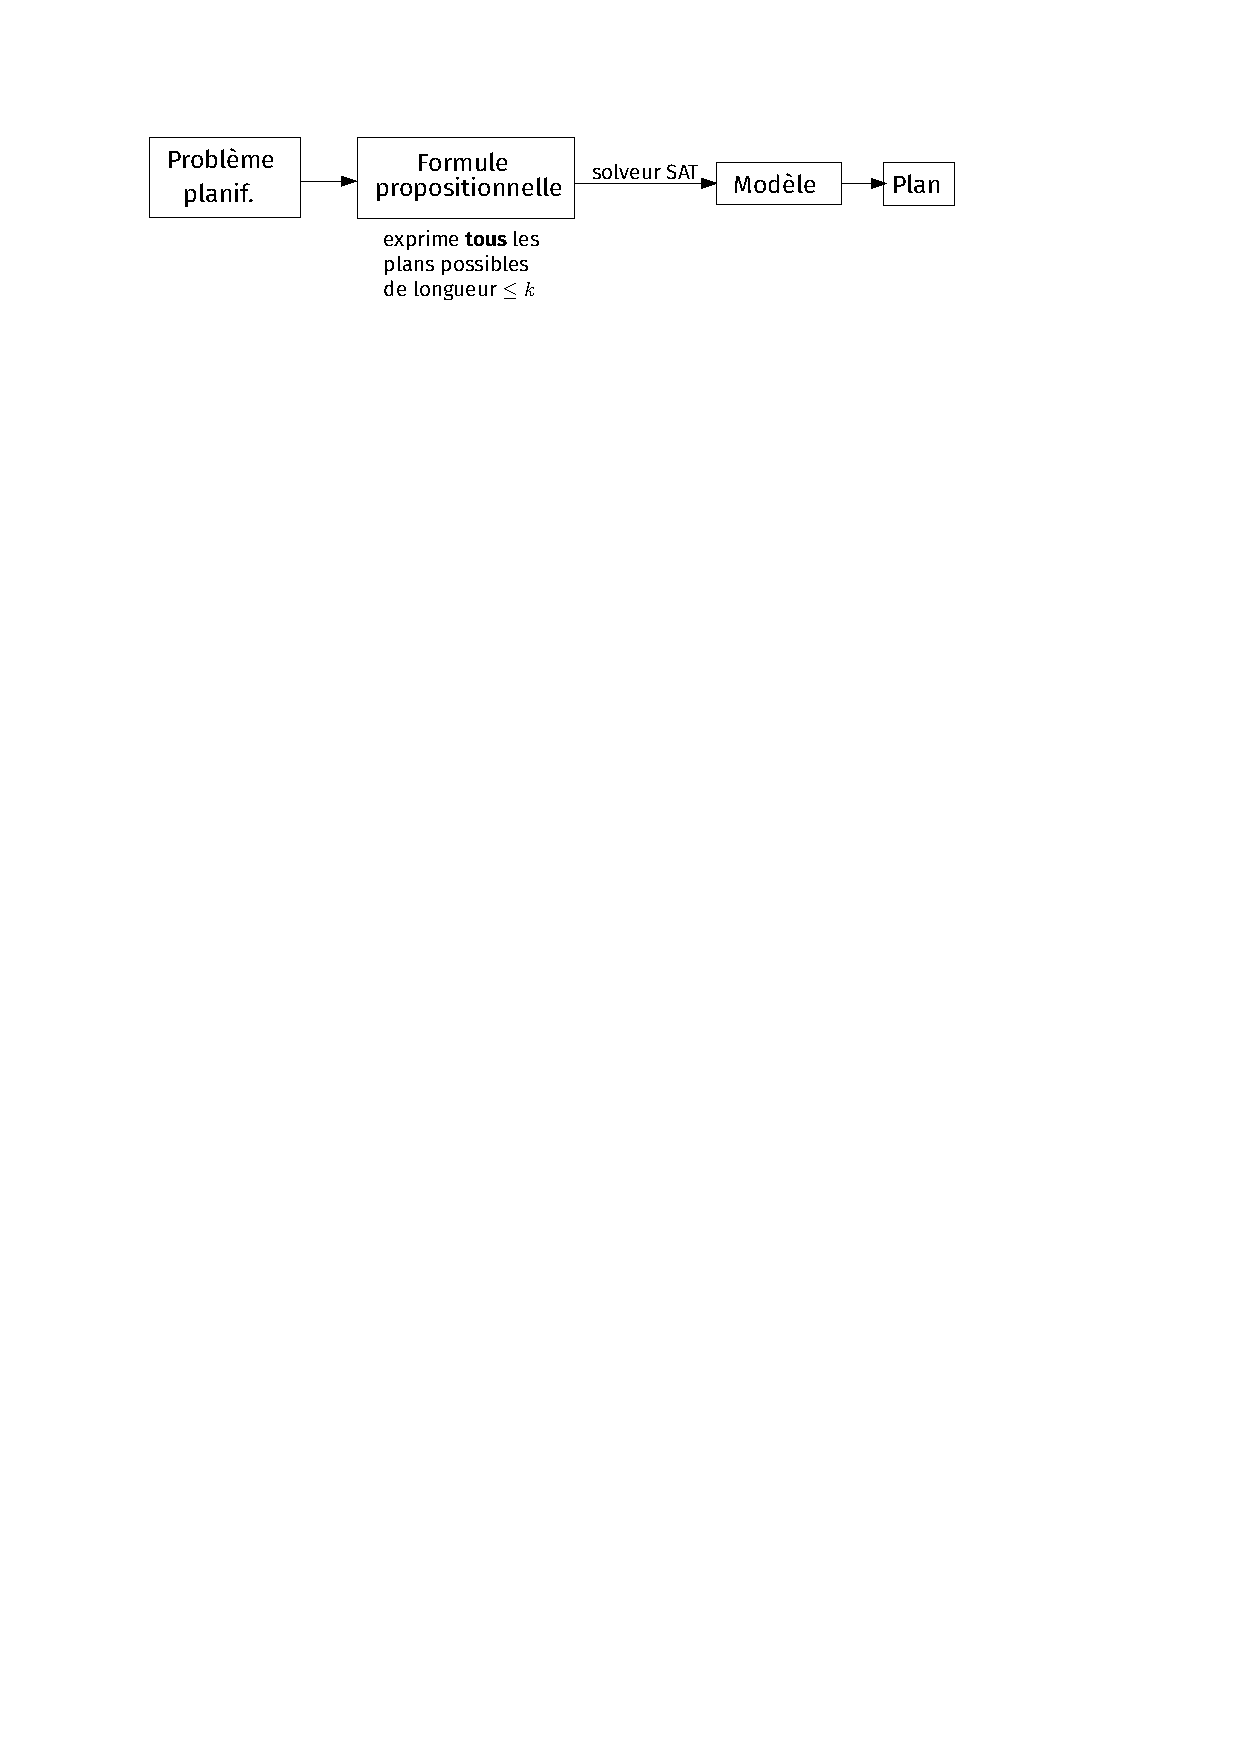
\includegraphics[width=0.98\paperwidth]{figures/coplas2018/planif-tree-1.pdf}}
\end{frame}

\begin{frame}
\makebox[\textwidth]{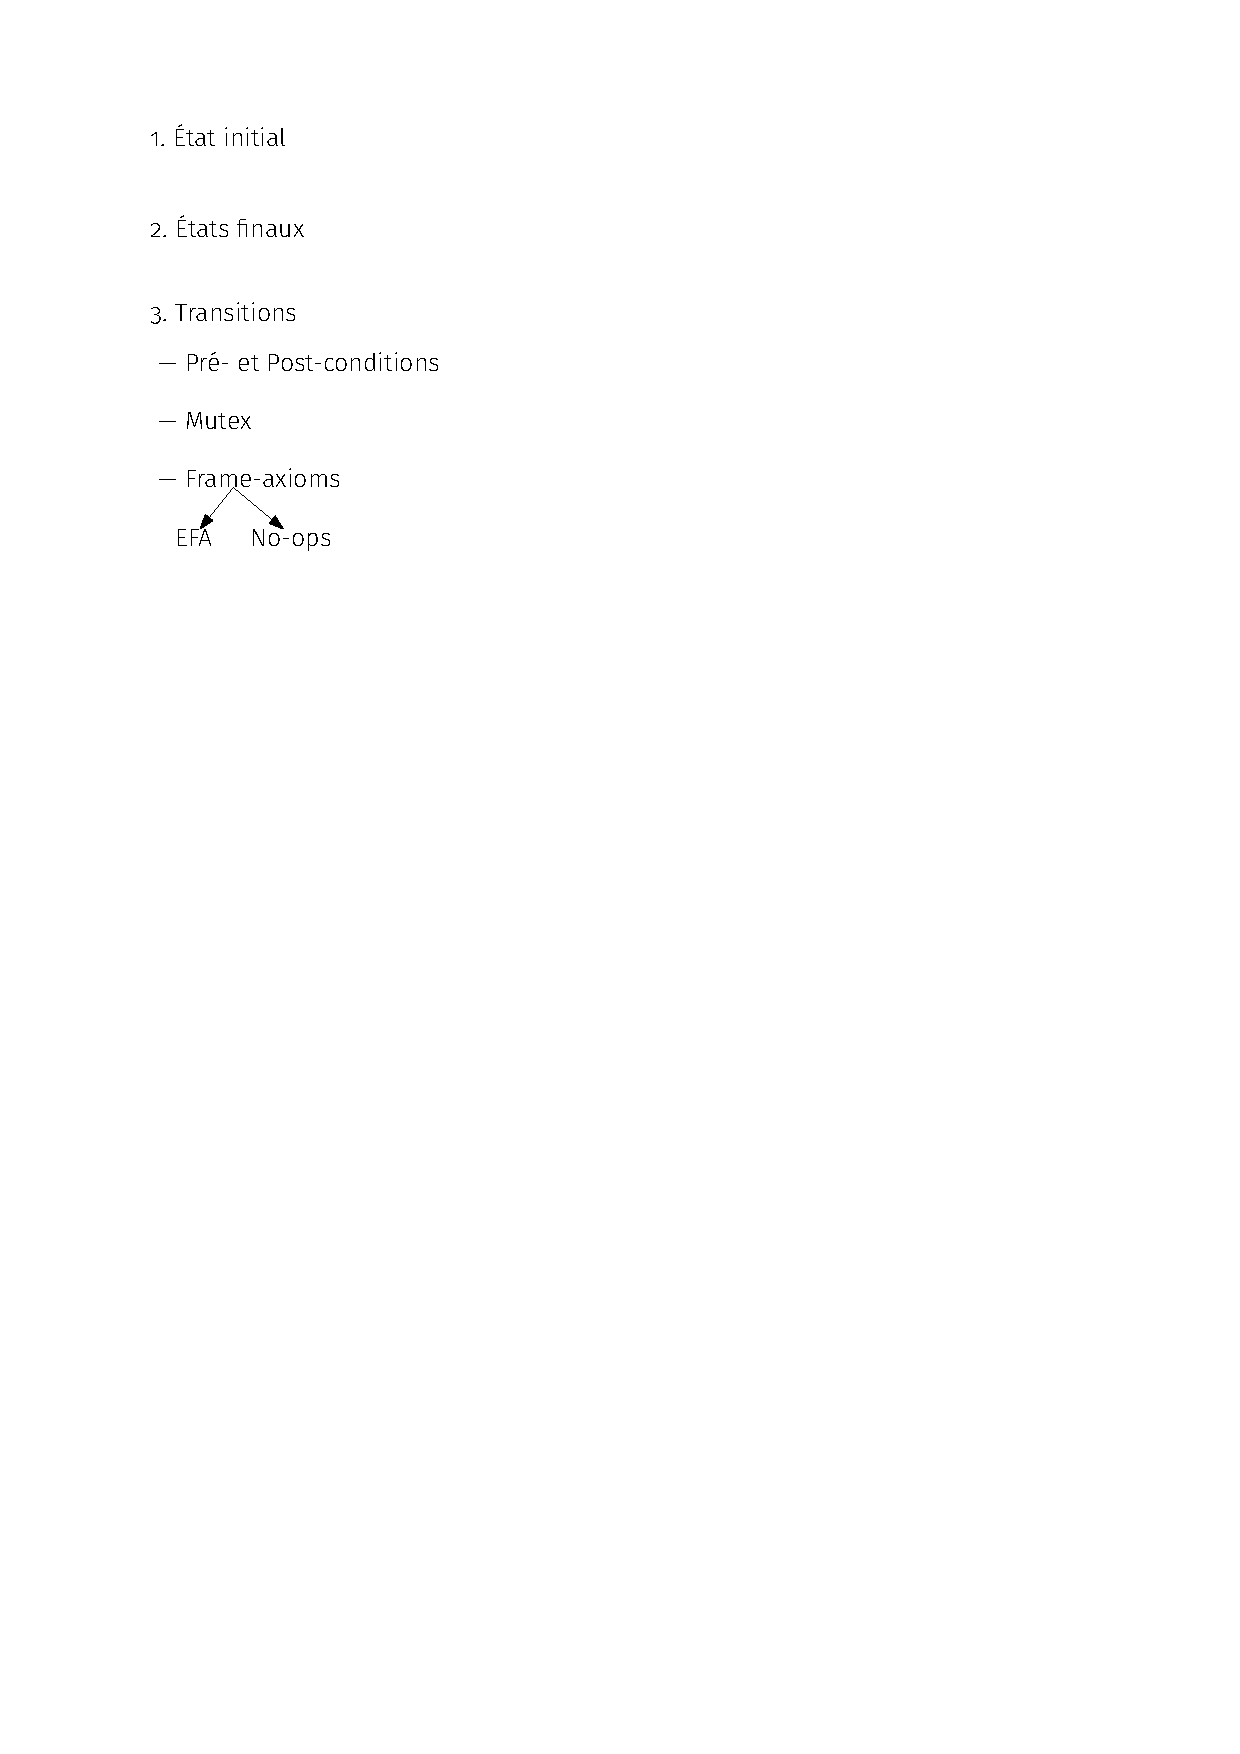
\includegraphics[width=0.9\paperwidth]{figures/coplas2018/planif-tree-2a.pdf}}    
\end{frame}
\begin{frame}
\makebox[\textwidth]{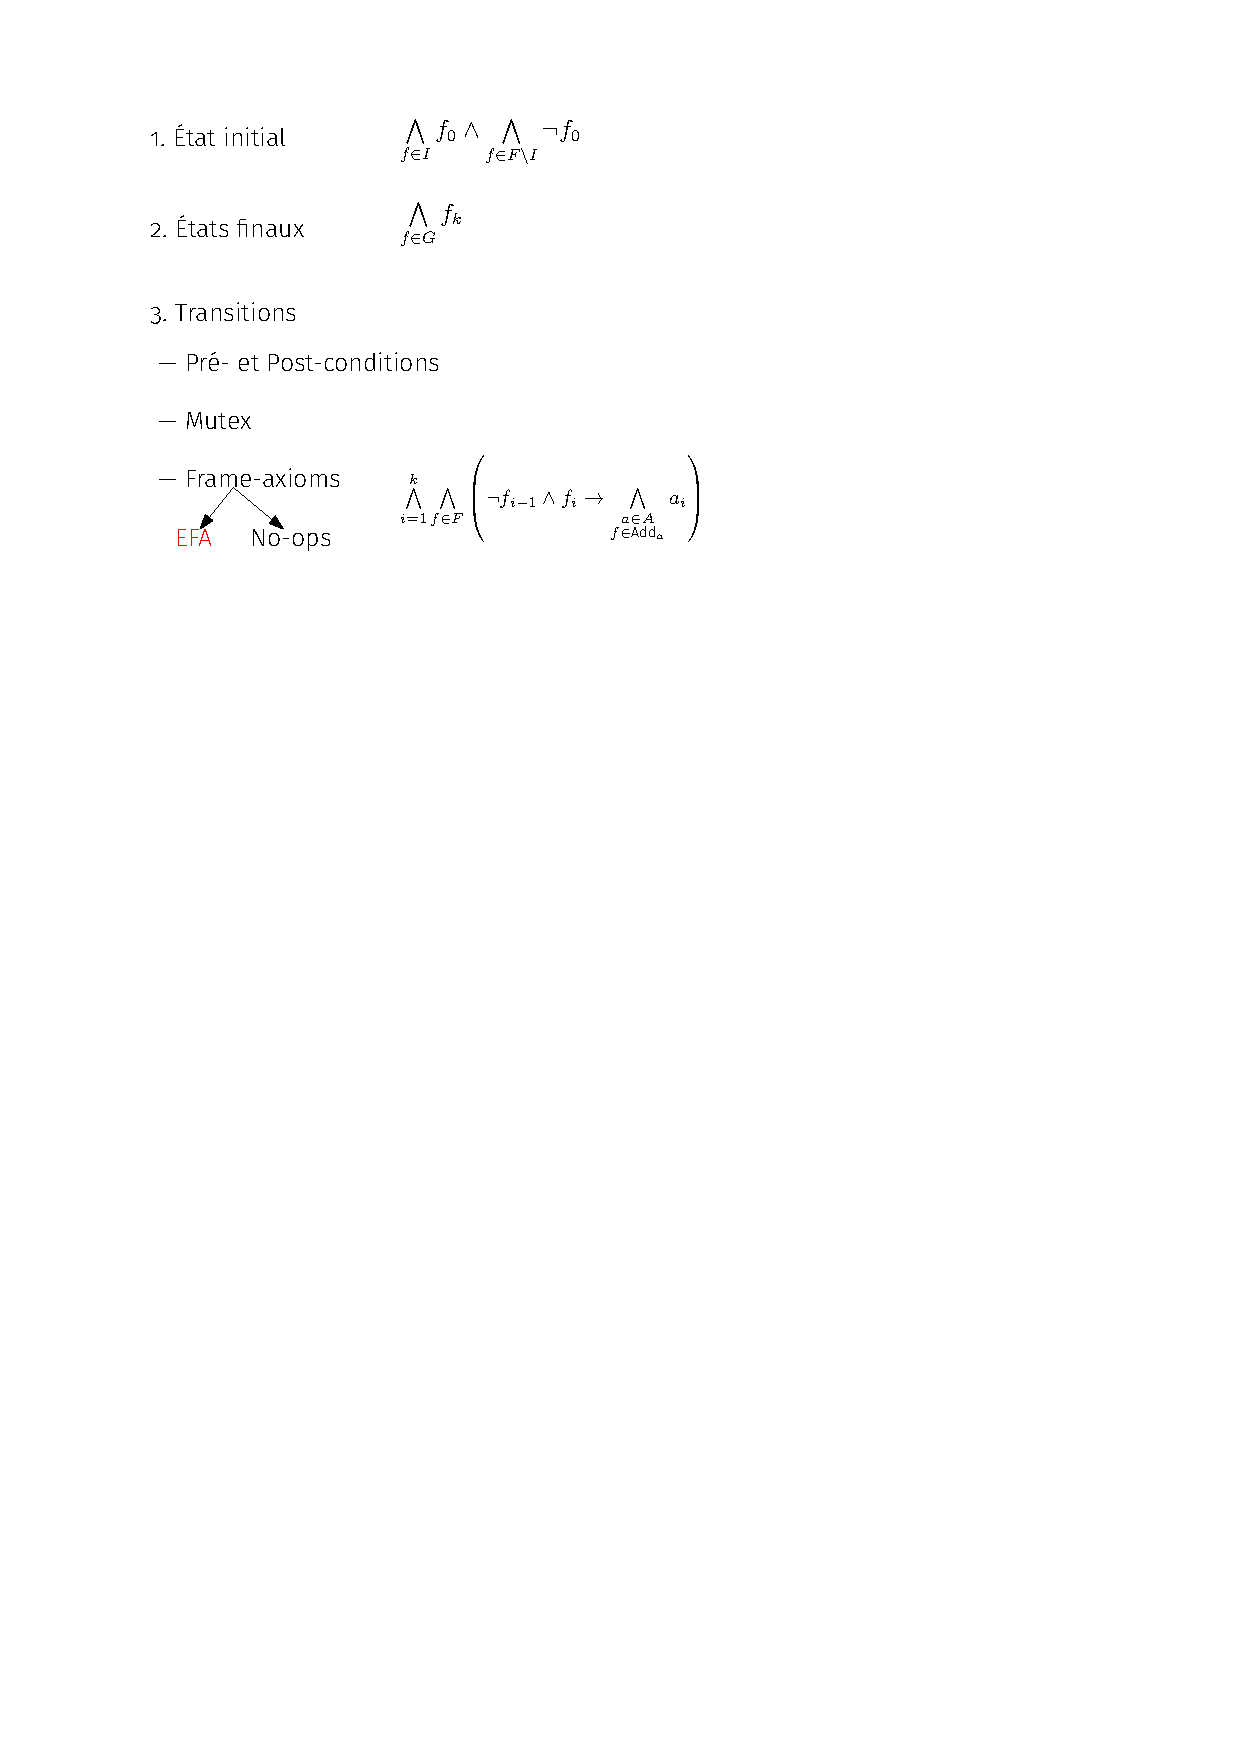
\includegraphics[width=0.9\paperwidth]{figures/coplas2018/planif-tree-2b.pdf}}    
\end{frame}
\begin{frame}
\makebox[\textwidth]{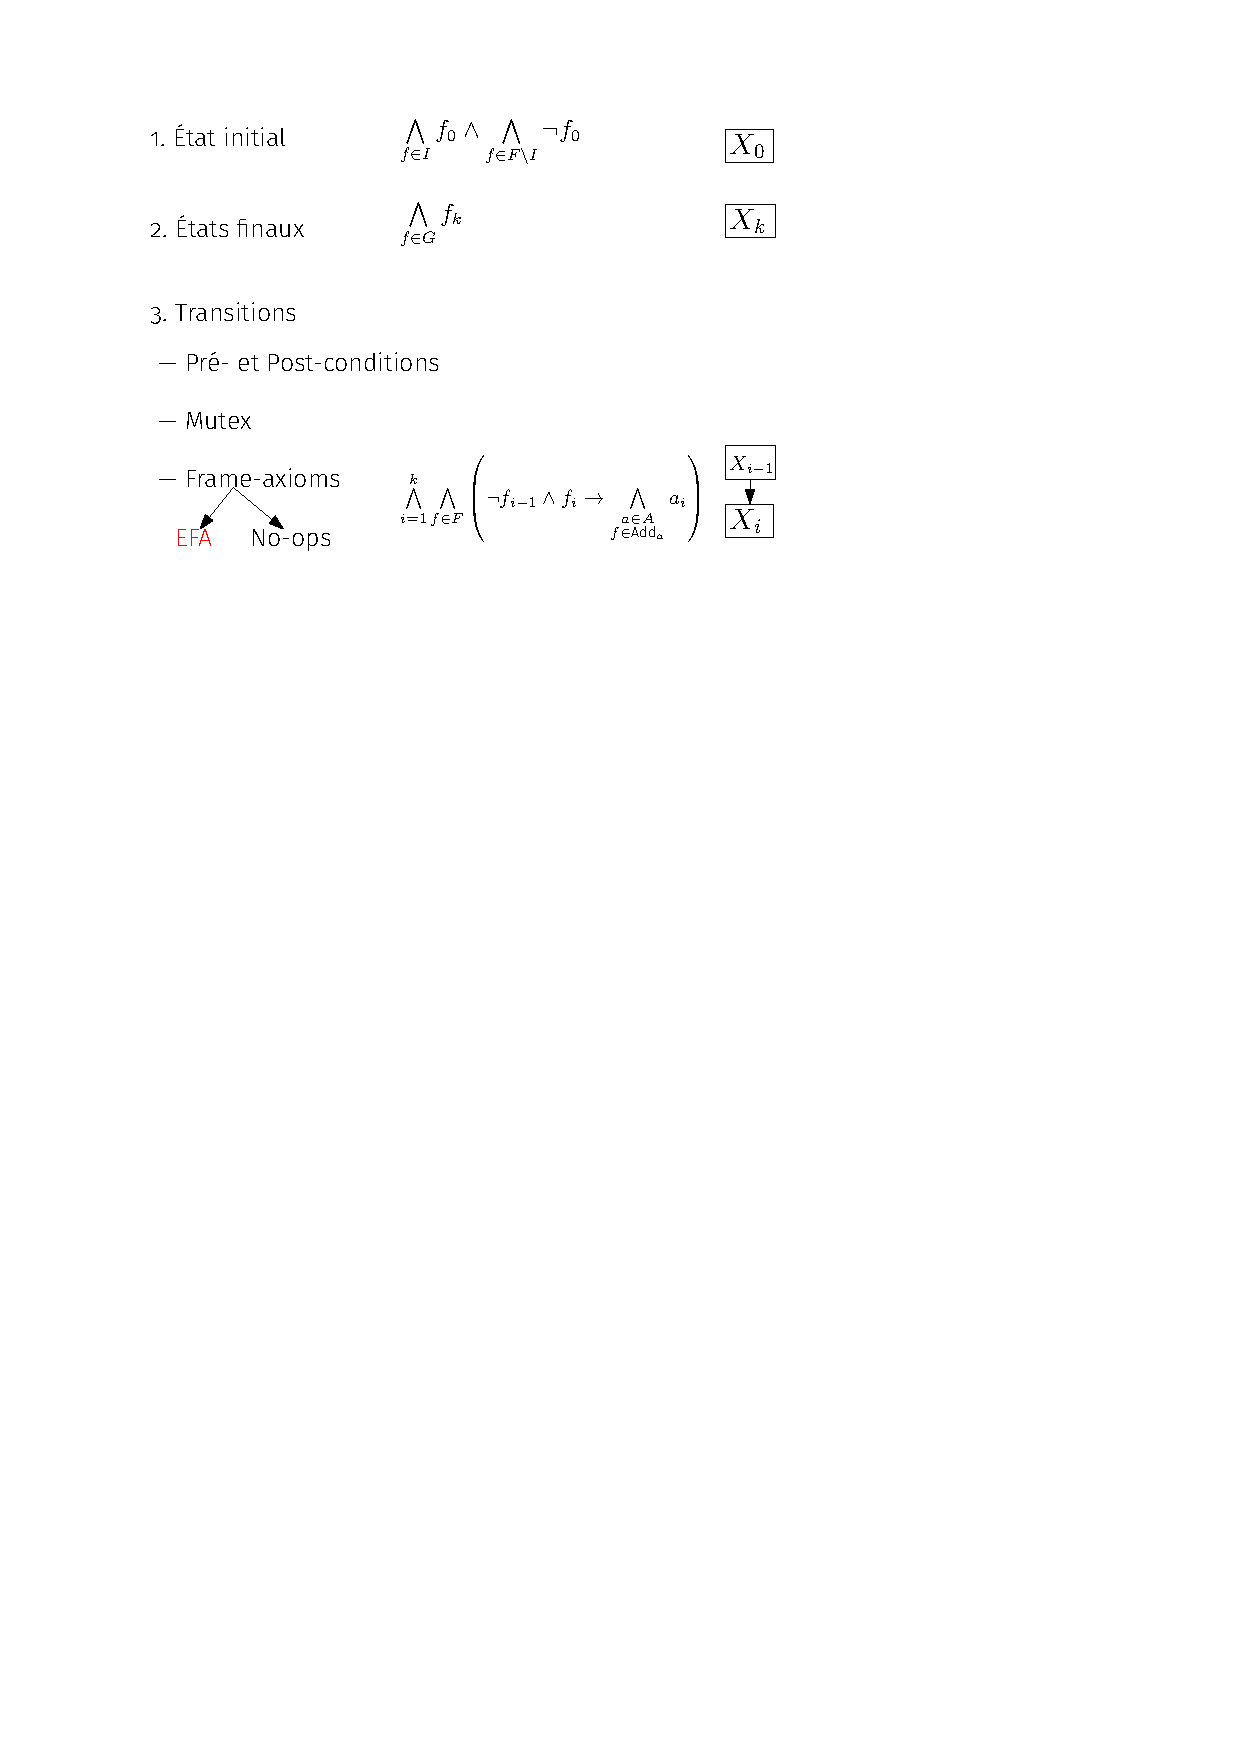
\includegraphics[width=0.9\paperwidth]{figures/coplas2018/planif-tree-2c.pdf}}    
\end{frame}


\begin{frame}{\subsecname}
\textbf{Étape 2} : passage en QBF
\begin{figure}
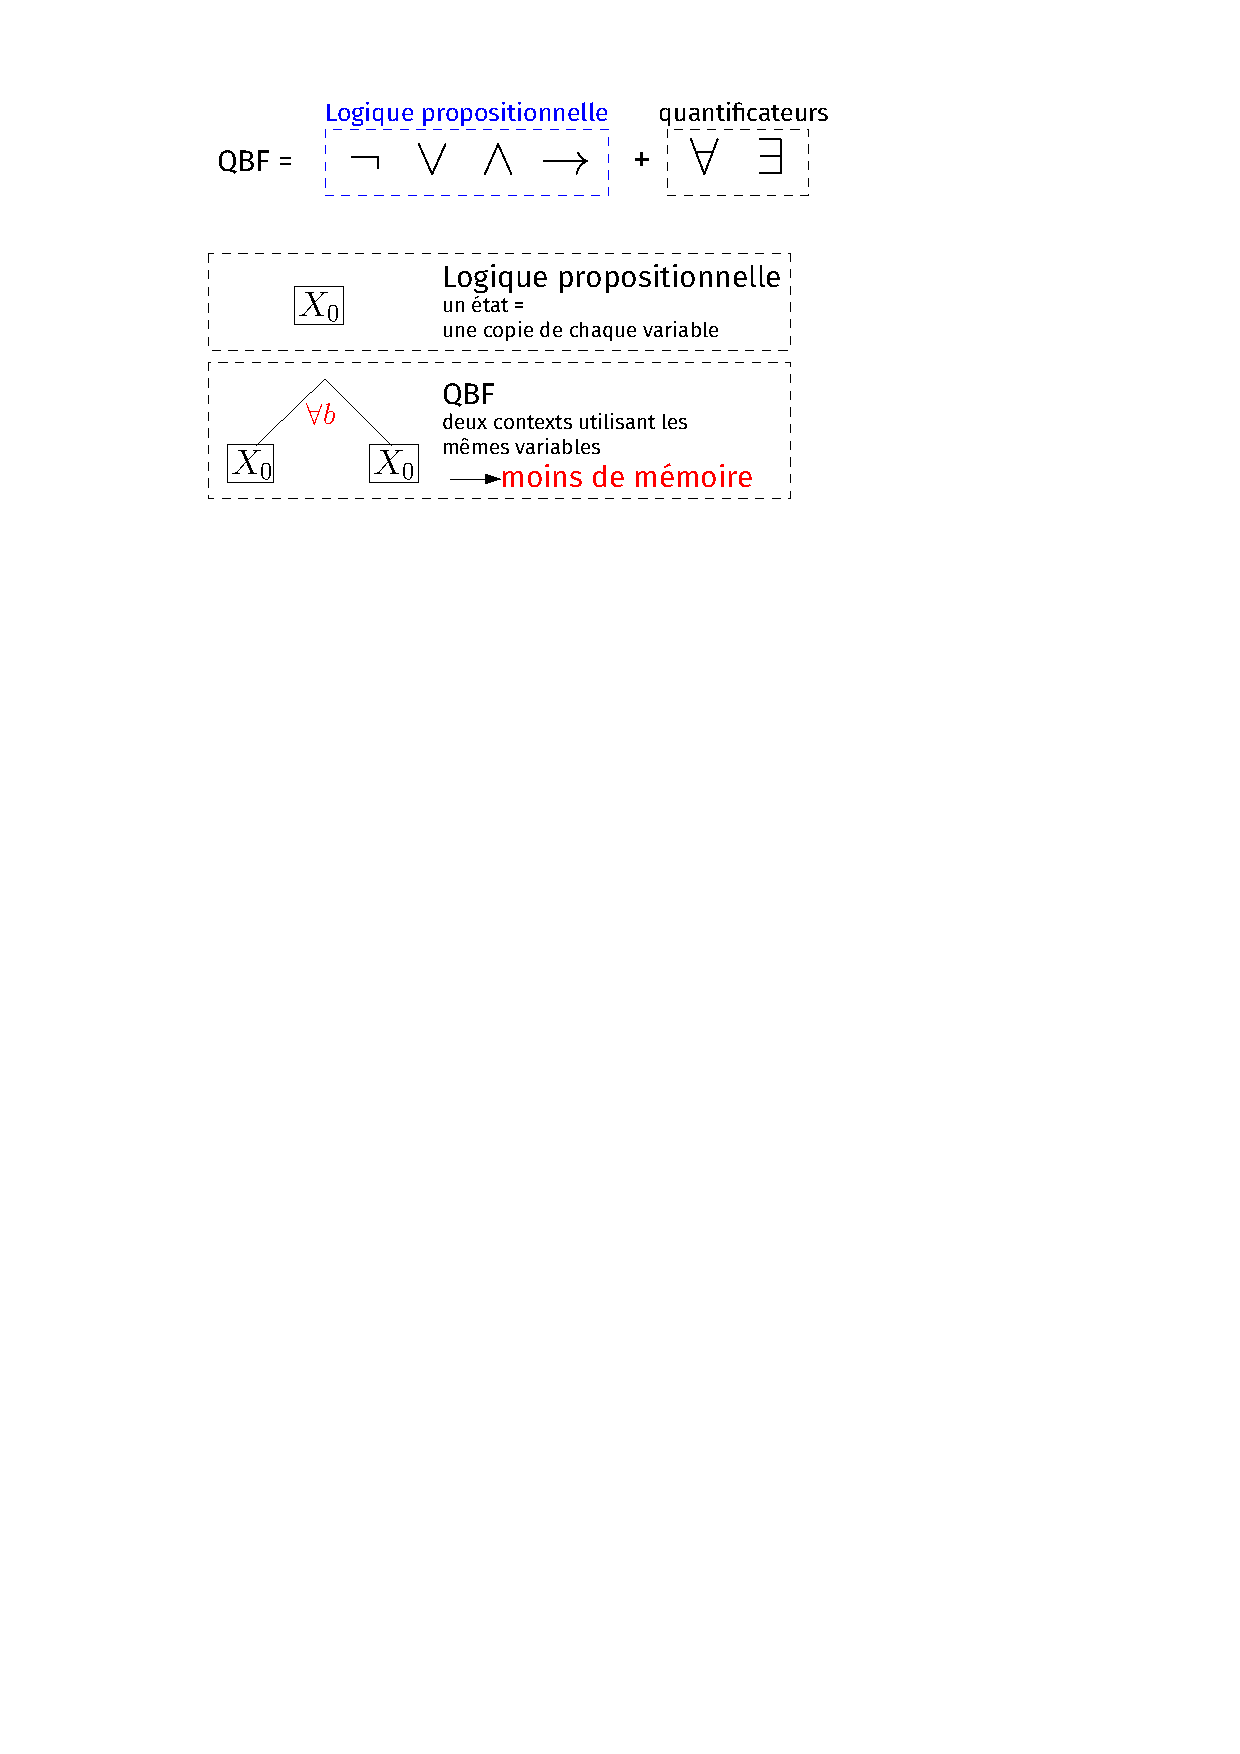
\includegraphics[width=0.9\textwidth]{figures/coplas2018/sat-vs-qbf.pdf}
\end{figure}
\end{frame}

\begin{frame}
\begin{center}\includegraphics[width=1\textwidth]{figures/coplas2018/planif-tree-2.pdf}\end{center}
$\longrightarrow$ Théoriquement, beaucoup \textbf{moins de mémoire} utilisée.
\end{frame}


\subsection{Exemple : le robot Gripper (planification QBF)}

\begin{frame}{\subsecname}
\begin{figure}[h]\label{gripper3:qbf-efa}
\begin{footnotesize}\xymatrix@C=-2.8pc@R=3pc{
   & & & & & *+[F]+{\substack{\grippermove{b}{a}}} \ar@{.}[lld]_{b_{2}=\bot} \ar@{.}[rrd]^{b_{2}=\top} \ar@/^1pc/[rdd] & & & & \\
   & & & *+[F]+{\substack{\grippermove{a}{b}}} \ar[rd]^{b_{1}=\top} & & & & *+[F]+{\substack{\grippermove{a}{b}}} \ar[rd]^{b_{1}=\top} & & \\
    & & *+[F]+{\substack{\gripperpick{1}{a}{left} \\ \gripperpick{3}{a}{right}}} \ar[ru]^{b_{1}=\bot}  & & *+[F]+{\substack{\gripperdrop{3}{b}{right}}} \ar@/^1pc/[ruu] & &  *+[F]+{\substack{\gripperpick{2}{a}{right}}} \ar[ru]^{b_{1}=\bot} & & *+[F]+{\substack{\gripperdrop{1}{b}{left}\\\gripperdrop{2}{b}{right}}} \\
}\end{footnotesize}
\caption{Transitions du plan en 7 étapes retourné par \touistplan{} pour le problème Gripper-3 (codage d'arbre compact QBF (CTE) de profondeur 2 dans les espaces d'états avec frame-axiomes explicatifs}
\end{figure}
Parcours infixe pour parcourir le plan.
\end{frame}



\begin{frame}
En pratique :
\begin{itemize}
\item En SAT, No-ops est la meilleure transition disponible
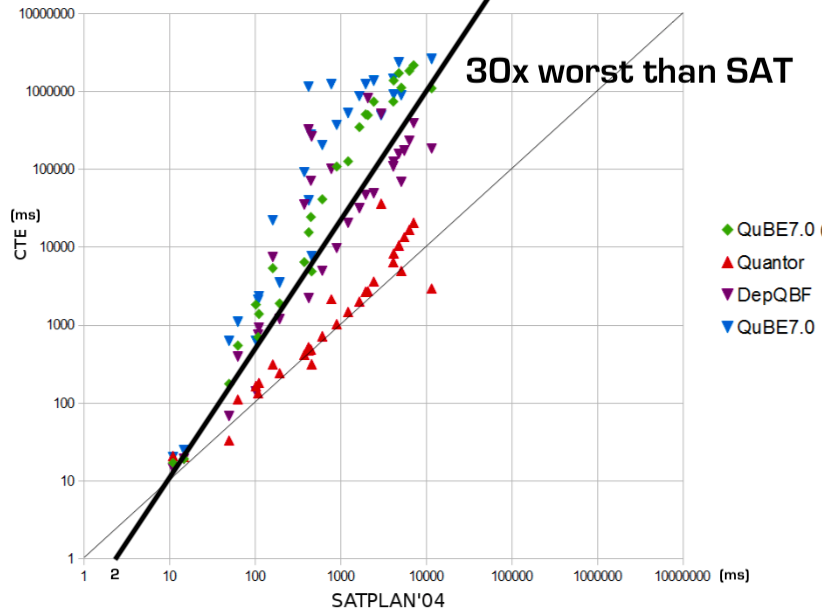
\includegraphics[width=0.6\textwidth]{figures/coplas2018/cashmore.png}
\item En QBF, No-ops utilise \textbf{5 $ \times $ moins de mémoire} mais \textbf{30 $ \times $ plus lent} (\cite{DBLP:conf/ecai/CashmoreFG12})
\end{itemize}
\end{frame}





\begin{frame}
\begin{exampleblock}{Question...}
Trouver meilleurs codages basés sur le CTE ?
\end{exampleblock}
\begin{alertblock}{Note}
Travail au niveau de l'encodage, {\color{red} pas au niveau solveur}
\end{alertblock}
\end{frame}


\subsection{Contribution : nouveaux codages pour résolution rapide}

\begin{frame}
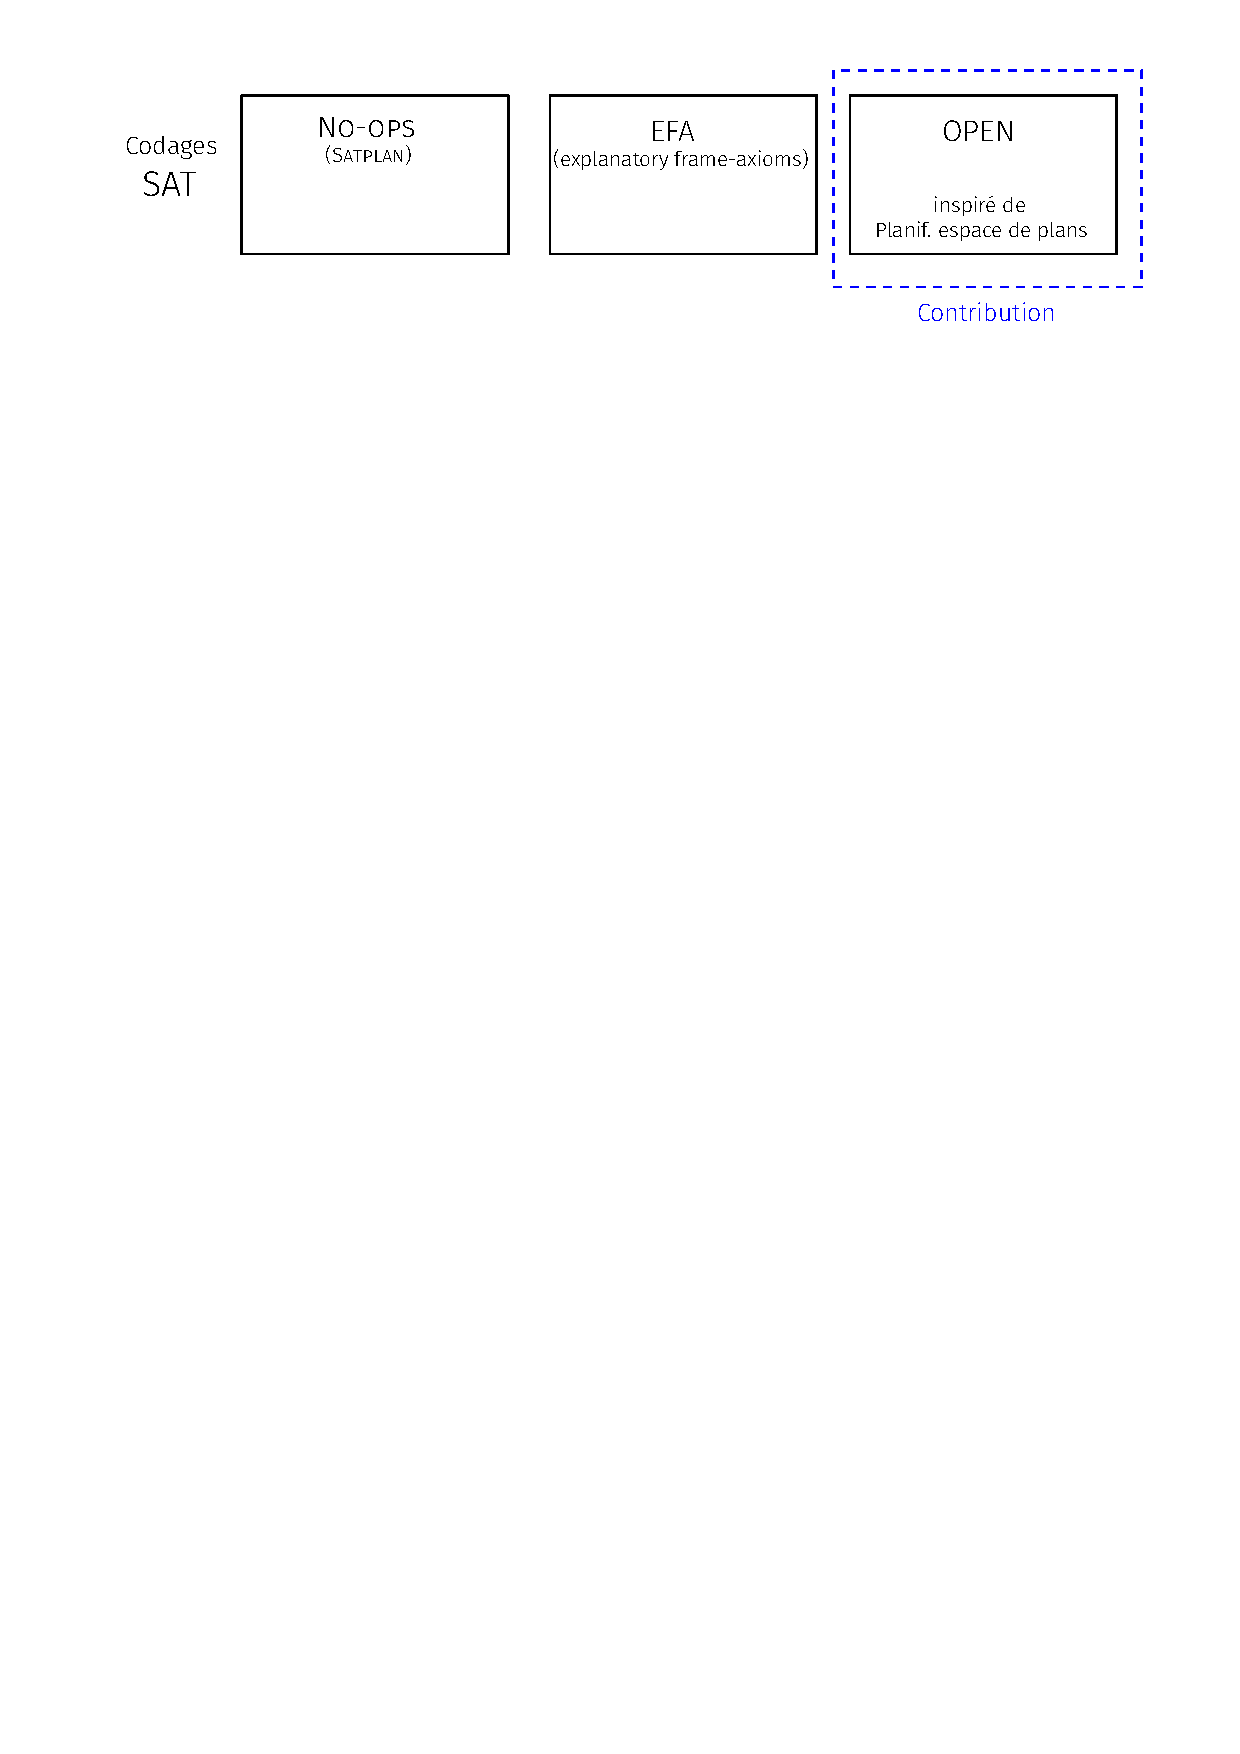
\includegraphics[width=1\textwidth]{figures/coplas2018/cte-encodings-1.pdf}
\end{frame}
\begin{frame}
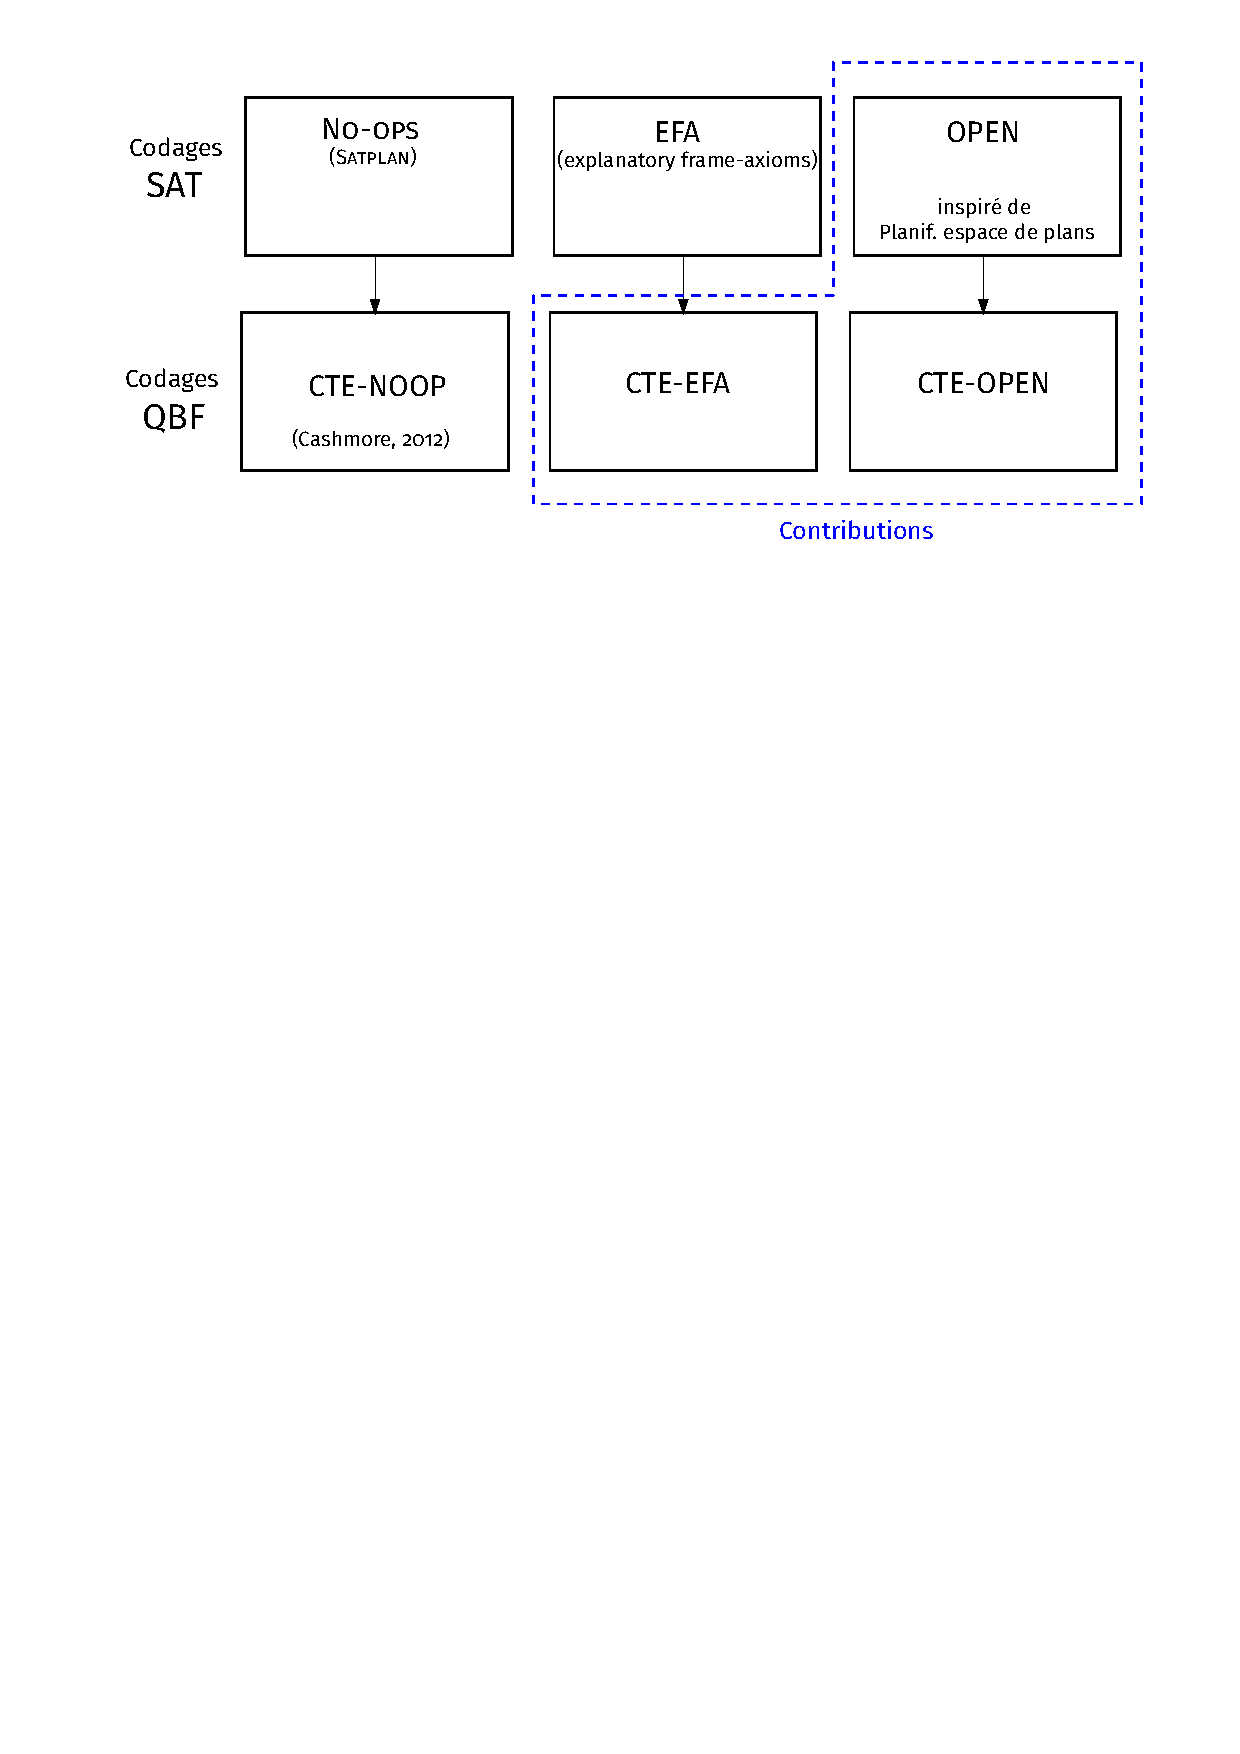
\includegraphics[width=1\textwidth]{figures/coplas2018/cte-encodings-2.pdf}
\end{frame}
\begin{frame}
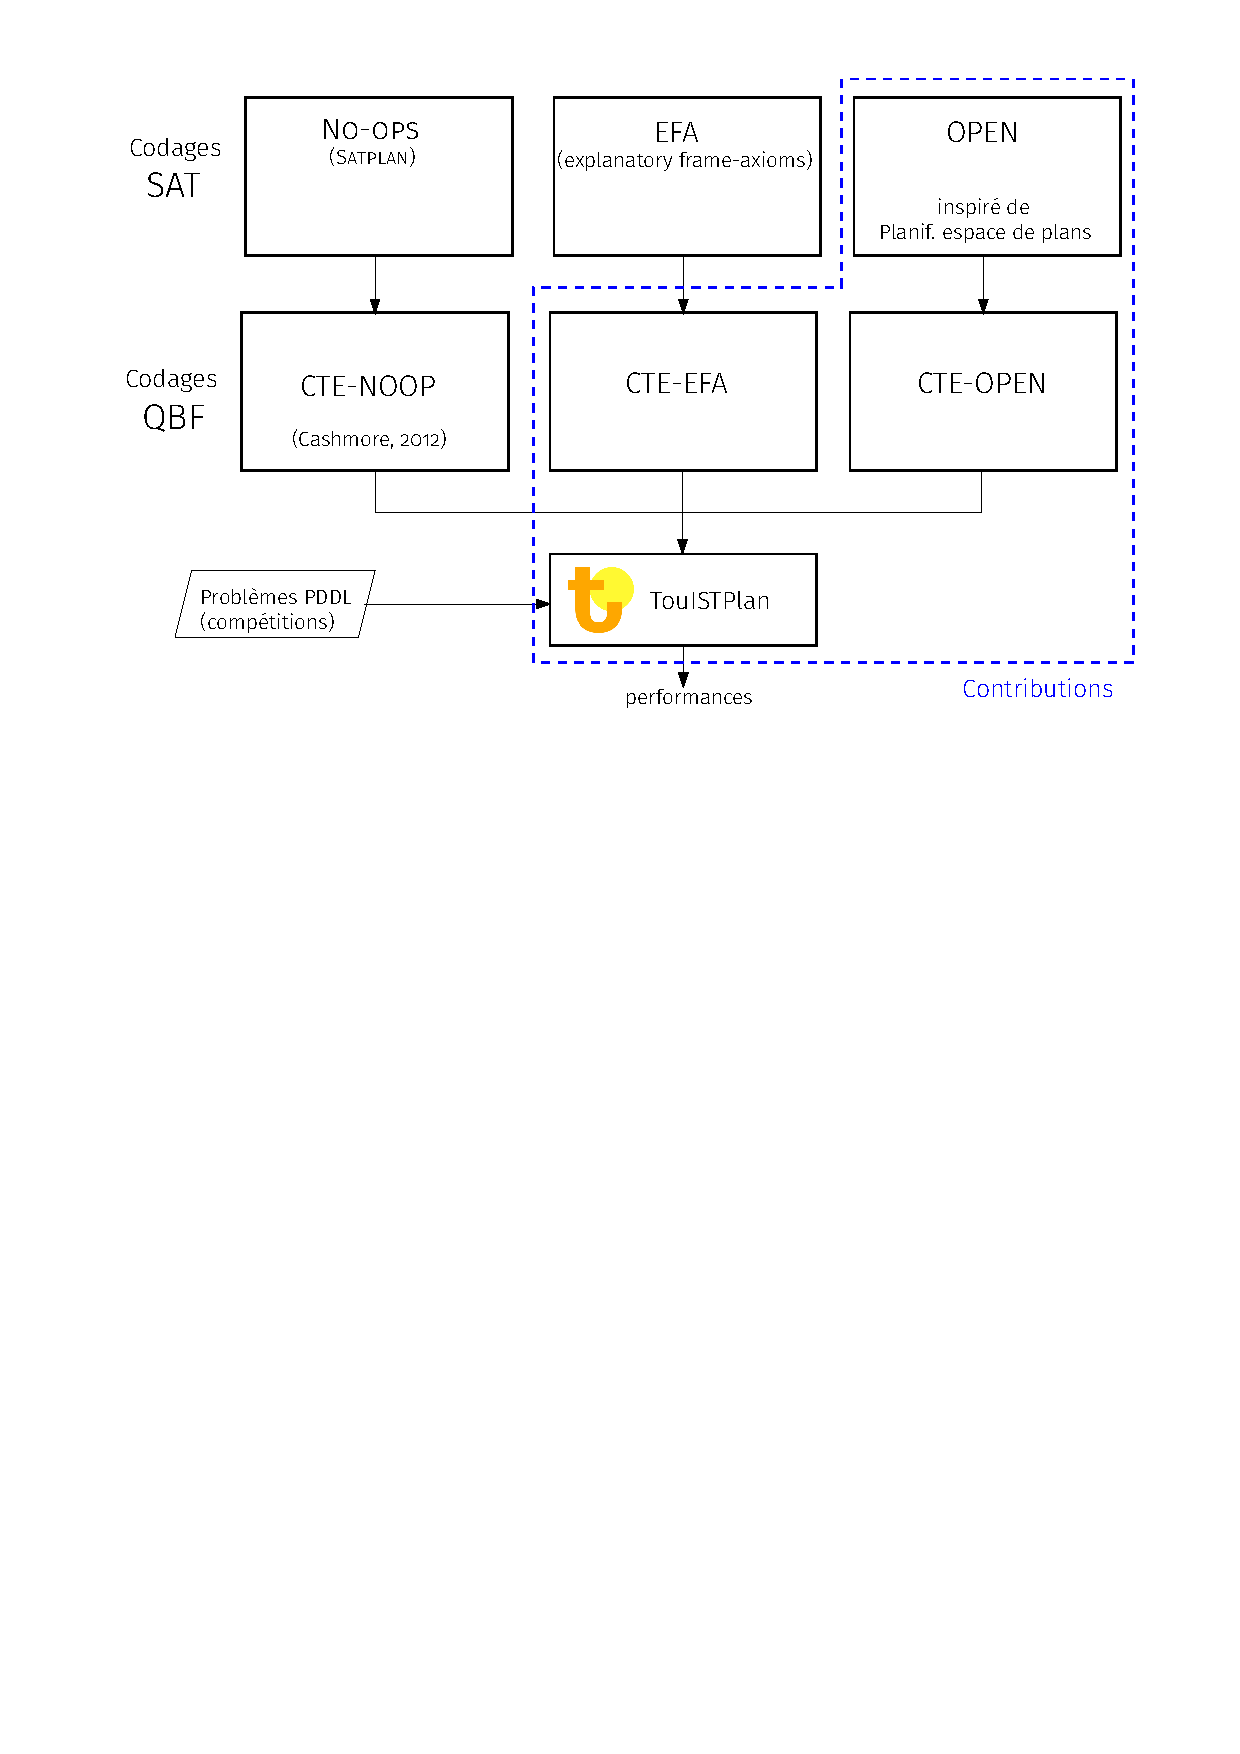
\includegraphics[width=1\textwidth]{figures/coplas2018/cte-encodings-3.pdf}
\end{frame}

\begin{frame}
\begin{itemize}

\item Utilise les domaines 1 à 8 des IPC (International  Planning Competition)
\item Solveurs QBF testés : RaREQS, DepQBF, Qute (Quantor trop lent)
\item {\color{red}6000 heures} de calcul (2112 problèmes à travers 3 solveurs)
\item Timeout de 1 heure pour le problème \textit{"y a-t-il un plan ?"}
\item Problèmes QBF générés en utilisant \textbf{TouIST} et \textbf{TouISTPlan}
\begin{itemize}
\item \url{https://github.com/touist/touistplan}

\includegraphics[width=0.6\textwidth]{figures/coplas2018/touist.png}
\end{itemize}
\end{itemize}
\end{frame}


\begin{frame}
Temps entre codages CTE pour le problème \textit{"y a-t-il un plan ?"} :

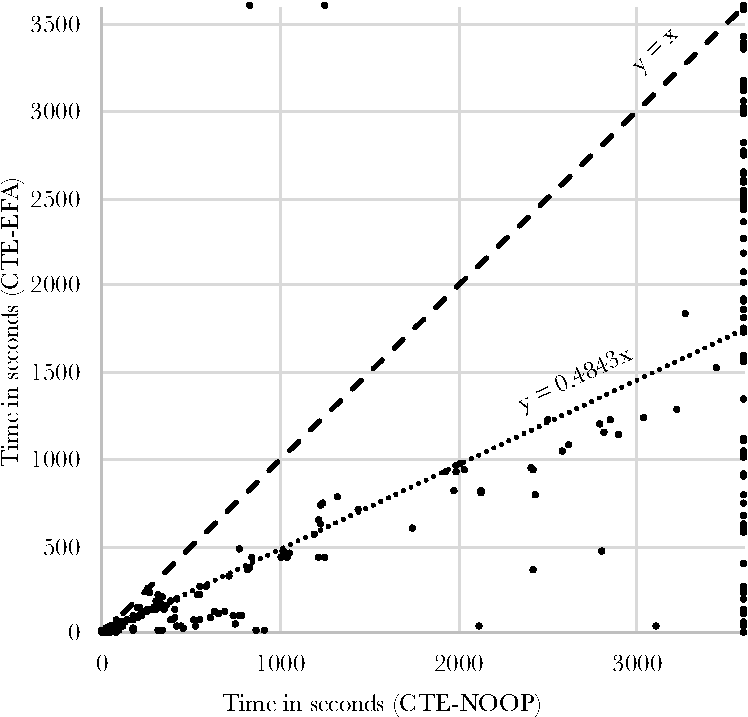
\includegraphics[width=0.5\textwidth]{figures/coplas2018/time-plansat-efa-noop3.pdf}
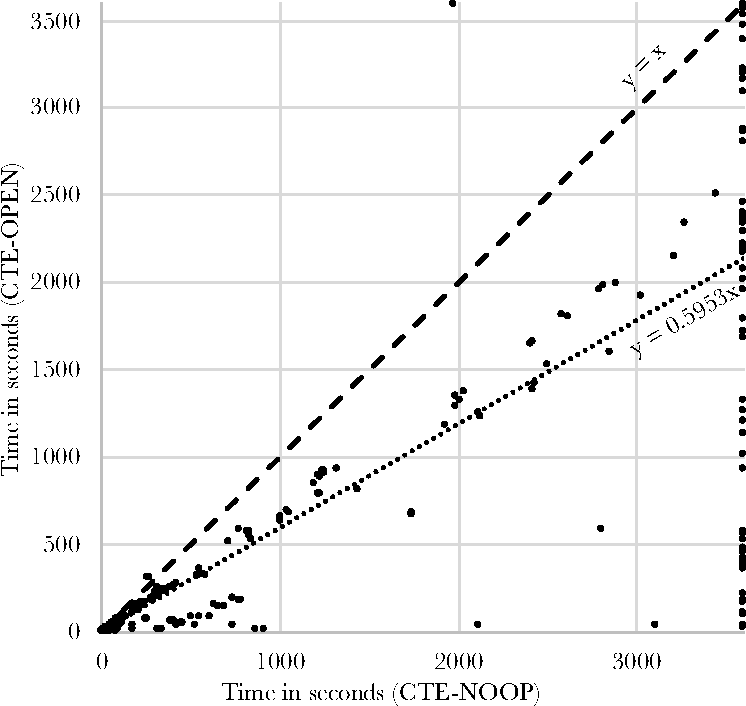
\includegraphics[width=0.5\textwidth]{figures/coplas2018/time-plansat-open-noop3.pdf}

\begin{columns}
\begin{column}{0.5\textwidth}
\begin{center}
CTE-OPEN est \textbf{1.7$\times$ plus rapide}
\end{center}
\end{column}
\begin{column}{0.5\textwidth}
\begin{center}
CTE-EFA est \textbf{2$\times$ plus rapide}
\end{center}
\end{column}
\end{columns}

\begin{small}\begin{center}
(comparé à CTE-NOOP)
\end{center} \end{small}
\begin{center}
De 30$\times$ à \textbf{seulement 15$\times$ moins rapide} que \textsc{Satplan}!
\end{center}
\end{frame}

\begin{frame}
\textbf{Petit souci technique}: on ne peut gérer qu'une profondeur de 3, càd \textbf{un plan d'une longueur de 15 étapes maximum} !
\begin{exampleblock}{Solution implémentée}
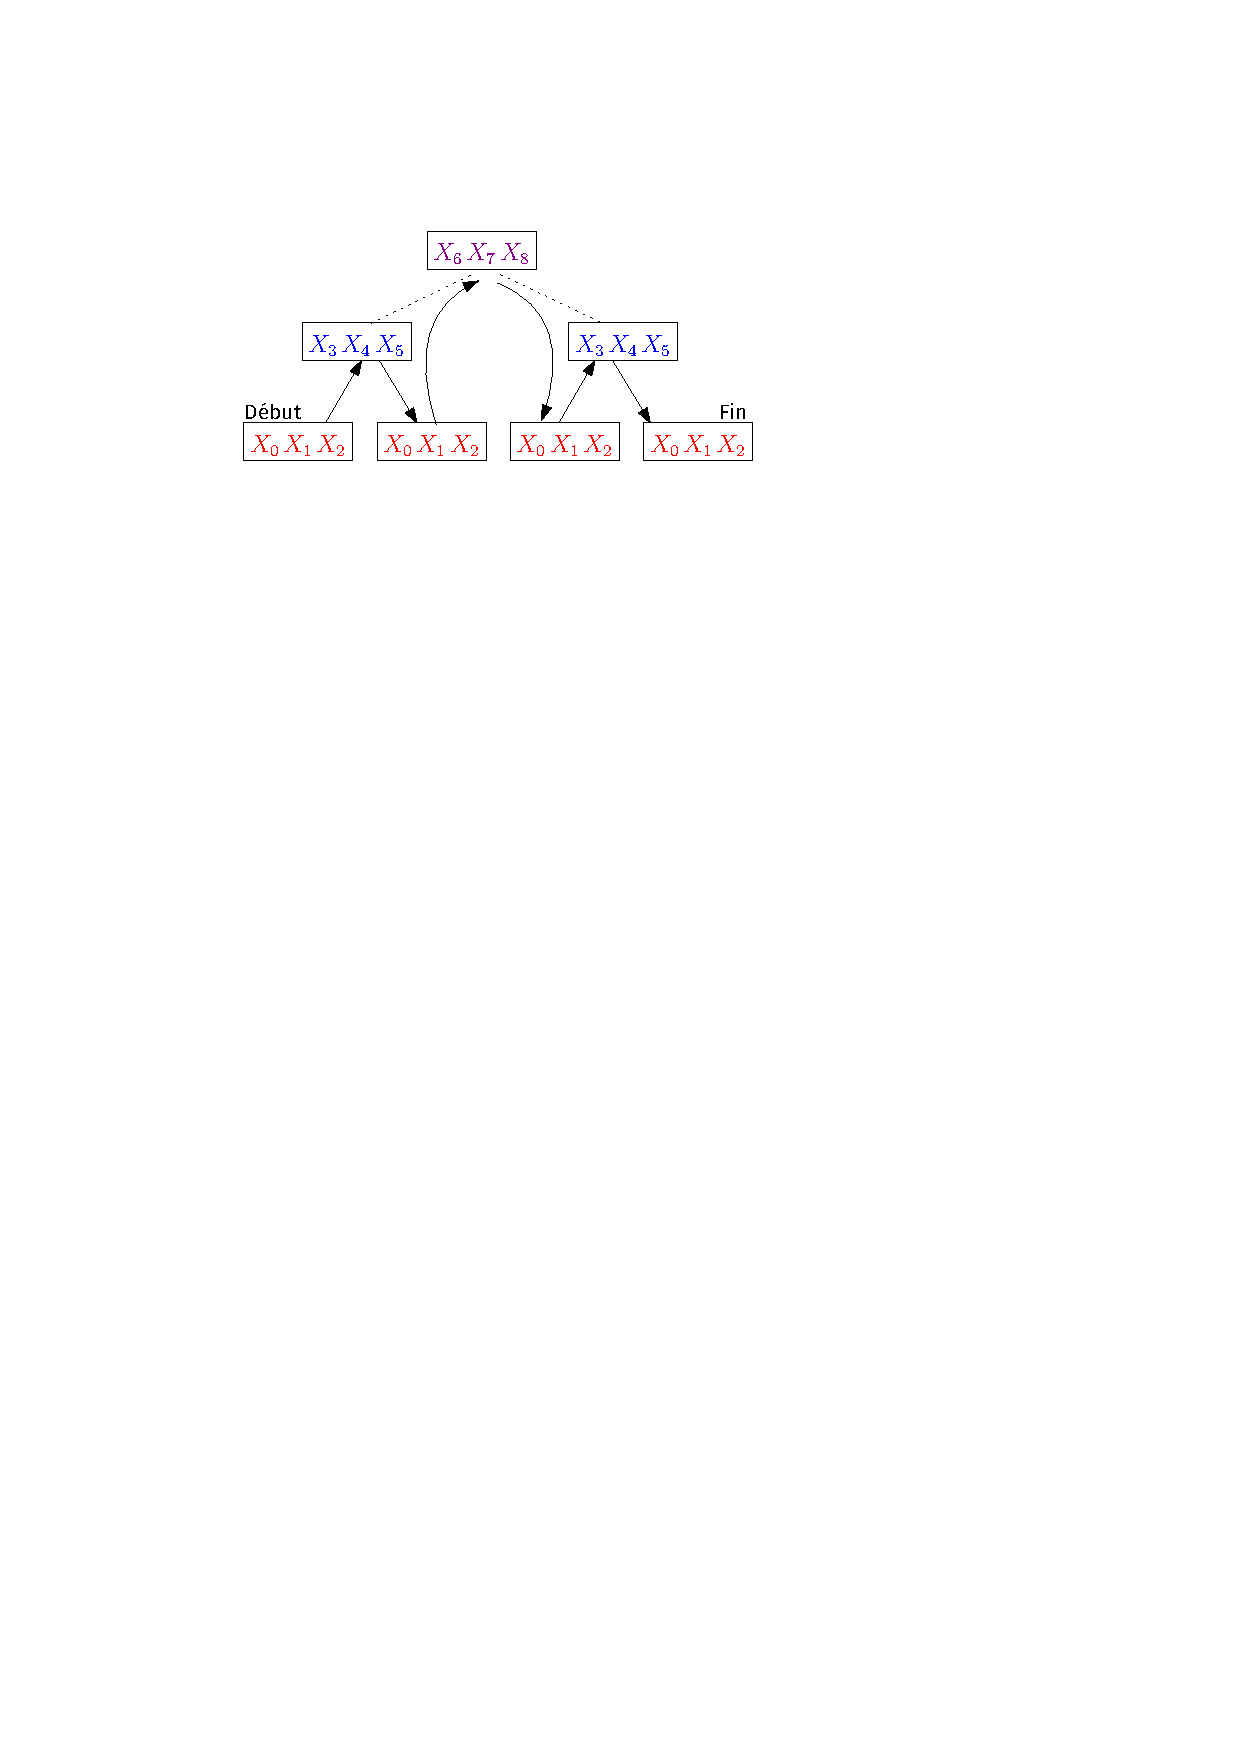
\includegraphics[width=\textwidth]{figures/coplas2018/planif-tree-5.pdf}
\end{exampleblock}
\end{frame}

\begin{frame}
Des métriques pour \textbf{expliquer} cette amélioration \textbf{$2\times$} ?
\begin{itemize}
\item Nombre de littéraux et nombre de clauses
\item Ratio entre les types de transitions (contraintes \textbf{branches} sur contraintes \textbf{nœuds})
\end{itemize}
\end{frame}

\begin{frame}
\begin{small}\begin{table} \centering
\begin{tabular}{@{}lccccc@{}}
\toprule
Codage & Nb résolus & Temps & Littéraux & Clauses & Ratio transitions \\ \midrule
CTE-NOOP & 412 (20\%) & 0\% & 0\% & 0\% & 30\% \\
CTE-EFA & 463 (22\%) & -55\% & -26\% & +15\% & 47\%  \\
CTE-OPEN & 445 (21\%) & -41\% & -2\% & -28\% & 17\% \\ \bottomrule \\
\end{tabular}
\end{table}\end{small}
Pas vraiment utile :
\begin{itemize}
\item Nombre de littéraux et nombre de clauses: {\color{red}pas de corrélation}
\item Types de transitions (nœuds/branches): {\color{red}pas de corrélation}
\end{itemize}
\end{frame}


\section*{Conclusion}

\begin{frame}{Contributions 1}
\textbf{Contributions liées à TouIST} :

\begin{itemize}
    \item Un outil et un langage, TouIST, améliorant l'expressivité pour utiliser les solveurs SAT, SMT et QBF pour l'enseignement et la recherche
    \item aide pour l'enseignement de la logique à l'université
    \begin{itemize} 
        \item[\plus] Étudiants de licence de l'Université Paul Sabatier
        \item[\plus] Étudiants de licence de l'\textbf{Université de Seville}
    \end{itemize}
    \item aide pour la recherche
    \begin{itemize} 
        \item[\plus] Codages pour la planification (IRIT, Toulouse)
        \item[\plus] Modélisation pour raisonnement épistémique (IRISA, Rennes)
    \end{itemize}
\end{itemize}
\end{frame}

\begin{frame}{Contributions 2}

\textbf{Contributions liées à la planification QBF} :
\begin{itemize}
\item[\plus] Un moyen systématique de \textbf{traduire les codages} depuis SAT vers QBF
\item[\plus] Par conséquence, deux nouveaux codage \textbf{plus performants que l'existant} (CTE-NOOP)
\item[\plus] Contribution d'un \textbf{large ensemble de benchmarks} générés à partir des problèmes IPC
\end{itemize}
\end{frame}

\begin{frame}{Perspectives}
\textbf{Perpectives liées à TouIST} :
\begin{itemize}
\item Finaliser TouIST "pour le web" pour favoriser l'adoption
\item utiliser TouIST pour la \textbf{planification épistémique} (DL-PA)
\item utiliser TouIST pour améliorer les performance de \textbf{LoTREC} (solveur de logiques modales)
\item utiliser TouIST pour améliorer \textbf{SESAME} (écriture de sémantiques argumentatives)
\end{itemize}
\end{frame}

\begin{frame}{Perspectives}
\textbf{Perpectives liées à la planification} :
\begin{itemize}
\item \textbf{Publication} de nos nouveaux benchmarks (à \textsc{QBFEVAL}) pour pousser les solveurs QBF à s'améliorer/se spécialiser dans ce domaine
\item Trouver \textbf{de meilleures métriques} permettant d'expliquer les améliorations et pouvoir les exploiter
\end{itemize}
\end{frame}

\bibliographystyle{apalike}
\bibliography{listrefs}
\end{document}